\documentclass[twoside]{book}

% Packages required by doxygen
\usepackage{fixltx2e}
\usepackage{calc}
\usepackage{doxygen}
\usepackage[export]{adjustbox} % also loads graphicx
\usepackage{graphicx}
\usepackage[utf8]{inputenc}
\usepackage{makeidx}
\usepackage{multicol}
\usepackage{multirow}
\PassOptionsToPackage{warn}{textcomp}
\usepackage{textcomp}
\usepackage[nointegrals]{wasysym}
\usepackage[table]{xcolor}

% Font selection
\usepackage[T1]{fontenc}
\usepackage[scaled=.90]{helvet}
\usepackage{courier}
\usepackage{amssymb}
\usepackage{sectsty}
\renewcommand{\familydefault}{\sfdefault}
\allsectionsfont{%
  \fontseries{bc}\selectfont%
  \color{darkgray}%
}
\renewcommand{\DoxyLabelFont}{%
  \fontseries{bc}\selectfont%
  \color{darkgray}%
}
\newcommand{\+}{\discretionary{\mbox{\scriptsize$\hookleftarrow$}}{}{}}

% Page & text layout
\usepackage{geometry}
\geometry{%
  a4paper,%
  top=2.5cm,%
  bottom=2.5cm,%
  left=2.5cm,%
  right=2.5cm%
}
\tolerance=750
\hfuzz=15pt
\hbadness=750
\setlength{\emergencystretch}{15pt}
\setlength{\parindent}{0cm}
\setlength{\parskip}{3ex plus 2ex minus 2ex}
\makeatletter
\renewcommand{\paragraph}{%
  \@startsection{paragraph}{4}{0ex}{-1.0ex}{1.0ex}{%
    \normalfont\normalsize\bfseries\SS@parafont%
  }%
}
\renewcommand{\subparagraph}{%
  \@startsection{subparagraph}{5}{0ex}{-1.0ex}{1.0ex}{%
    \normalfont\normalsize\bfseries\SS@subparafont%
  }%
}
\makeatother

% Headers & footers
\usepackage{fancyhdr}
\pagestyle{fancyplain}
\fancyhead[LE]{\fancyplain{}{\bfseries\thepage}}
\fancyhead[CE]{\fancyplain{}{}}
\fancyhead[RE]{\fancyplain{}{\bfseries\leftmark}}
\fancyhead[LO]{\fancyplain{}{\bfseries\rightmark}}
\fancyhead[CO]{\fancyplain{}{}}
\fancyhead[RO]{\fancyplain{}{\bfseries\thepage}}
\fancyfoot[LE]{\fancyplain{}{}}
\fancyfoot[CE]{\fancyplain{}{}}
\fancyfoot[RE]{\fancyplain{}{\bfseries\scriptsize Generated by Doxygen }}
\fancyfoot[LO]{\fancyplain{}{\bfseries\scriptsize Generated by Doxygen }}
\fancyfoot[CO]{\fancyplain{}{}}
\fancyfoot[RO]{\fancyplain{}{}}
\renewcommand{\footrulewidth}{0.4pt}
\renewcommand{\chaptermark}[1]{%
  \markboth{#1}{}%
}
\renewcommand{\sectionmark}[1]{%
  \markright{\thesection\ #1}%
}

% Indices & bibliography
\usepackage{natbib}
\usepackage[titles]{tocloft}
\setcounter{tocdepth}{3}
\setcounter{secnumdepth}{5}
\makeindex

% Hyperlinks (required, but should be loaded last)
\usepackage{ifpdf}
\ifpdf
  \usepackage[pdftex,pagebackref=true]{hyperref}
\else
  \usepackage[ps2pdf,pagebackref=true]{hyperref}
\fi
\hypersetup{%
  colorlinks=true,%
  linkcolor=blue,%
  citecolor=blue,%
  unicode%
}

% Custom commands
\newcommand{\clearemptydoublepage}{%
  \newpage{\pagestyle{empty}\cleardoublepage}%
}

\usepackage{caption}
\captionsetup{labelsep=space,justification=centering,font={bf},singlelinecheck=off,skip=4pt,position=top}

%===== C O N T E N T S =====

\begin{document}

% Titlepage & ToC
\hypersetup{pageanchor=false,
             bookmarksnumbered=true,
             pdfencoding=unicode
            }
\pagenumbering{roman}
\begin{titlepage}
\vspace*{7cm}
\begin{center}%
{\Large My Project }\\
\vspace*{1cm}
{\large Generated by Doxygen 1.8.11}\\
\end{center}
\end{titlepage}
\clearemptydoublepage
\tableofcontents
\clearemptydoublepage
\pagenumbering{arabic}
\hypersetup{pageanchor=true}

%--- Begin generated contents ---
\chapter{Class Index}
\section{Class List}
Here are the classes, structs, unions and interfaces with brief descriptions\+:\begin{DoxyCompactList}
\item\contentsline{section}{\hyperlink{structarrayd}{arrayd} }{\pageref{structarrayd}}{}
\item\contentsline{section}{\hyperlink{structarraytagnum}{arraytagnum} }{\pageref{structarraytagnum}}{}
\item\contentsline{section}{\hyperlink{structdate}{date} }{\pageref{structdate}}{}
\item\contentsline{section}{\hyperlink{structduplo}{duplo} }{\pageref{structduplo}}{}
\item\contentsline{section}{\hyperlink{structheap}{heap} }{\pageref{structheap}}{}
\item\contentsline{section}{\hyperlink{structheapu}{heapu} }{\pageref{structheapu}}{}
\item\contentsline{section}{\hyperlink{structkey}{key} }{\pageref{structkey}}{}
\item\contentsline{section}{\hyperlink{structllist}{llist} }{\pageref{structllist}}{}
\item\contentsline{section}{\hyperlink{structlong__pair}{long\+\_\+pair} }{\pageref{structlong__pair}}{}
\item\contentsline{section}{\hyperlink{structpost}{post} }{\pageref{structpost}}{}
\item\contentsline{section}{\hyperlink{structrespostas}{respostas} }{\pageref{structrespostas}}{}
\item\contentsline{section}{\hyperlink{structstr__pair}{str\+\_\+pair} }{\pageref{structstr__pair}}{}
\item\contentsline{section}{\hyperlink{structtag}{tag} }{\pageref{structtag}}{}
\item\contentsline{section}{\hyperlink{structtagnum}{tagnum} }{\pageref{structtagnum}}{}
\item\contentsline{section}{\hyperlink{structTCD__community}{T\+C\+D\+\_\+community} }{\pageref{structTCD__community}}{}
\item\contentsline{section}{\hyperlink{structuser}{user} }{\pageref{structuser}}{}
\item\contentsline{section}{\hyperlink{structuserint}{userint} }{\pageref{structuserint}}{}
\end{DoxyCompactList}

\chapter{File Index}
\section{File List}
Here is a list of all documented files with brief descriptions\+:\begin{DoxyCompactList}
\item\contentsline{section}{lib/\hyperlink{arrayT_8c}{array\+T.\+c} \\*Ficheiro que contém a implementação de um Array com uma \hyperlink{structtag}{tag(char$\ast$)} e o número de ocorrências }{\pageref{arrayT_8c}}{}
\item\contentsline{section}{lib/\hyperlink{heap_8c}{heap.\+c} \\*Ficheiro que contém a implementação de Max Heap\textquotesingle{}s de Posts }{\pageref{heap_8c}}{}
\item\contentsline{section}{lib/\hyperlink{heapU_8c}{heap\+U.\+c} \\*Ficheiro que contém a implementação de Max Heap\textquotesingle{}s }{\pageref{heapU_8c}}{}
\item\contentsline{section}{lib/\hyperlink{key_8c}{key.\+c} \\*Ficheiro que contem a implementação de Keys. Uma Key é um apontador para um long }{\pageref{key_8c}}{}
\item\contentsline{section}{lib/\hyperlink{mypost_8c}{mypost.\+c} \\*Ficheiro que contém a implementação de Posts }{\pageref{mypost_8c}}{}
\item\contentsline{section}{lib/\hyperlink{mytags_8c}{mytags.\+c} \\*Ficheiro que contém a implementação das Tags }{\pageref{mytags_8c}}{}
\item\contentsline{section}{lib/\hyperlink{util_8c}{util.\+c} \\*Ficheiro que contém a implementação de estruturas e funções úteis para resolução de querys }{\pageref{util_8c}}{}
\end{DoxyCompactList}

\chapter{Class Documentation}
\hypertarget{structarrayd}{}\section{arrayd Struct Reference}
\label{structarrayd}\index{arrayd@{arrayd}}
\subsection*{Public Attributes}
\begin{DoxyCompactItemize}
\item 
Post $\ast$ {\bfseries array}\hypertarget{structarrayd_a3910603430a073ecbda589dd2a238ca6}{}\label{structarrayd_a3910603430a073ecbda589dd2a238ca6}

\item 
long {\bfseries used}\hypertarget{structarrayd_a0dfc8a8e91a318beff11fbed6c8b1d29}{}\label{structarrayd_a0dfc8a8e91a318beff11fbed6c8b1d29}

\item 
long {\bfseries size}\hypertarget{structarrayd_ae4e9730ae4d0e45afa341644eff6f4d2}{}\label{structarrayd_ae4e9730ae4d0e45afa341644eff6f4d2}

\item 
long {\bfseries res}\hypertarget{structarrayd_aaf8038f3334c07bf90bf4f0858b27605}{}\label{structarrayd_aaf8038f3334c07bf90bf4f0858b27605}

\item 
long {\bfseries per}\hypertarget{structarrayd_ac95ef34a26b4246fdf4f0ef5c0e79008}{}\label{structarrayd_ac95ef34a26b4246fdf4f0ef5c0e79008}

\end{DoxyCompactItemize}


The documentation for this struct was generated from the following file\+:\begin{DoxyCompactItemize}
\item 
lib/\hyperlink{mypost_8c}{mypost.\+c}\end{DoxyCompactItemize}

\hypertarget{structarraytagnum}{}\section{arraytagnum Struct Reference}
\label{structarraytagnum}\index{arraytagnum@{arraytagnum}}
\subsection*{Public Attributes}
\begin{DoxyCompactItemize}
\item 
long {\bfseries size}\hypertarget{structarraytagnum_af422161be6f3cc894fa3b171ff9f4f8b}{}\label{structarraytagnum_af422161be6f3cc894fa3b171ff9f4f8b}

\item 
long {\bfseries used}\hypertarget{structarraytagnum_ad4468371ac12208b0fd5f3fdb1678c19}{}\label{structarraytagnum_ad4468371ac12208b0fd5f3fdb1678c19}

\item 
T\+Num $\ast$ {\bfseries tags}\hypertarget{structarraytagnum_ad8ba5aa2dc3010ea277c465ee099bd2e}{}\label{structarraytagnum_ad8ba5aa2dc3010ea277c465ee099bd2e}

\end{DoxyCompactItemize}


The documentation for this struct was generated from the following file\+:\begin{DoxyCompactItemize}
\item 
lib/\hyperlink{arrayT_8c}{array\+T.\+c}\end{DoxyCompactItemize}

\hypertarget{structdate}{}\section{date Struct Reference}
\label{structdate}\index{date@{date}}
\subsection*{Public Attributes}
\begin{DoxyCompactItemize}
\item 
int {\bfseries day}\hypertarget{structdate_a2649784269c2be62800d1e4509ed2b56}{}\label{structdate_a2649784269c2be62800d1e4509ed2b56}

\item 
int {\bfseries month}\hypertarget{structdate_a4007efea3f7afe04e9a195dc13f71f38}{}\label{structdate_a4007efea3f7afe04e9a195dc13f71f38}

\item 
int {\bfseries year}\hypertarget{structdate_a12304556327d9ea913a0534a8554107a}{}\label{structdate_a12304556327d9ea913a0534a8554107a}

\end{DoxyCompactItemize}


The documentation for this struct was generated from the following file\+:\begin{DoxyCompactItemize}
\item 
lib/date.\+c\end{DoxyCompactItemize}

\hypertarget{structduplo}{}\section{duplo Struct Reference}
\label{structduplo}\index{duplo@{duplo}}
\subsection*{Public Attributes}
\begin{DoxyCompactItemize}
\item 
L\+O\+N\+G\+\_\+list {\bfseries ll}\hypertarget{structduplo_ab8f2e221e0498f8fdffb15e476d24496}{}\label{structduplo_ab8f2e221e0498f8fdffb15e476d24496}

\item 
T\+Num {\bfseries tnum}\hypertarget{structduplo_a96309c6acf504637d0b13d6bb0b5f2db}{}\label{structduplo_a96309c6acf504637d0b13d6bb0b5f2db}

\item 
int {\bfseries pos}\hypertarget{structduplo_a961c7fa25d1753417ad3eb7621868a38}{}\label{structduplo_a961c7fa25d1753417ad3eb7621868a38}

\end{DoxyCompactItemize}


The documentation for this struct was generated from the following file\+:\begin{DoxyCompactItemize}
\item 
lib/\hyperlink{util_8c}{util.\+c}\end{DoxyCompactItemize}

\hypertarget{structheap}{}\section{heap Struct Reference}
\label{structheap}\index{heap@{heap}}
\subsection*{Public Attributes}
\begin{DoxyCompactItemize}
\item 
int {\bfseries tamanho}\hypertarget{structheap_a5b2c9d7ad6862b4b98761d3c18bf21de}{}\label{structheap_a5b2c9d7ad6862b4b98761d3c18bf21de}

\item 
int {\bfseries pos}\hypertarget{structheap_a7098a64af665b5f0d18f8c3f718ece90}{}\label{structheap_a7098a64af665b5f0d18f8c3f718ece90}

\item 
char $\ast$ {\bfseries pal}\hypertarget{structheap_a894049ec19e81366f11906dbd6743646}{}\label{structheap_a894049ec19e81366f11906dbd6743646}

\item 
Post $\ast$ {\bfseries posts}\hypertarget{structheap_a06d20d32f9d12beb273fcd412e18006d}{}\label{structheap_a06d20d32f9d12beb273fcd412e18006d}

\end{DoxyCompactItemize}


The documentation for this struct was generated from the following file\+:\begin{DoxyCompactItemize}
\item 
lib/\hyperlink{heap_8c}{heap.\+c}\end{DoxyCompactItemize}

\hypertarget{structheapu}{}\section{heapu Struct Reference}
\label{structheapu}\index{heapu@{heapu}}
\subsection*{Public Attributes}
\begin{DoxyCompactItemize}
\item 
long {\bfseries tamanho}\hypertarget{structheapu_ab8d72282b1c88bb0b3ade563554a6406}{}\label{structheapu_ab8d72282b1c88bb0b3ade563554a6406}

\item 
long {\bfseries pos}\hypertarget{structheapu_a608fbc33b10960925a1263da99b2dcdd}{}\label{structheapu_a608fbc33b10960925a1263da99b2dcdd}

\item 
long $\ast$ {\bfseries qnt}\hypertarget{structheapu_a8d50b7cfee48359dab683d3057099398}{}\label{structheapu_a8d50b7cfee48359dab683d3057099398}

\item 
long $\ast$ {\bfseries ids}\hypertarget{structheapu_a214bffde83b4ad51860e610edd675cca}{}\label{structheapu_a214bffde83b4ad51860e610edd675cca}

\end{DoxyCompactItemize}


The documentation for this struct was generated from the following file\+:\begin{DoxyCompactItemize}
\item 
lib/\hyperlink{heapU_8c}{heap\+U.\+c}\end{DoxyCompactItemize}

\hypertarget{structkey}{}\section{key Struct Reference}
\label{structkey}\index{key@{key}}
\subsection*{Public Attributes}
\begin{DoxyCompactItemize}
\item 
long {\bfseries key}\hypertarget{structkey_a2498705c24e7e286c7ce54961a1417e3}{}\label{structkey_a2498705c24e7e286c7ce54961a1417e3}

\end{DoxyCompactItemize}


The documentation for this struct was generated from the following file\+:\begin{DoxyCompactItemize}
\item 
lib/\hyperlink{key_8c}{key.\+c}\end{DoxyCompactItemize}

\hypertarget{structllist}{}\section{llist Struct Reference}
\label{structllist}\index{llist@{llist}}
\subsection*{Public Attributes}
\begin{DoxyCompactItemize}
\item 
int {\bfseries size}\hypertarget{structllist_a10e612886a406b85ba87caefa8dd7e4e}{}\label{structllist_a10e612886a406b85ba87caefa8dd7e4e}

\item 
long $\ast$ {\bfseries list}\hypertarget{structllist_a47b4d503f0df6354f20154b58ef0d7f1}{}\label{structllist_a47b4d503f0df6354f20154b58ef0d7f1}

\end{DoxyCompactItemize}


The documentation for this struct was generated from the following file\+:\begin{DoxyCompactItemize}
\item 
lib/list.\+c\end{DoxyCompactItemize}

\hypertarget{structlong__pair}{}\section{long\+\_\+pair Struct Reference}
\label{structlong__pair}\index{long\+\_\+pair@{long\+\_\+pair}}
\subsection*{Public Attributes}
\begin{DoxyCompactItemize}
\item 
long {\bfseries fst}\hypertarget{structlong__pair_a7cfd71dae8a1bff732fbf8a372129327}{}\label{structlong__pair_a7cfd71dae8a1bff732fbf8a372129327}

\item 
long {\bfseries snd}\hypertarget{structlong__pair_ac6845698d9c04e20c768f12181598503}{}\label{structlong__pair_ac6845698d9c04e20c768f12181598503}

\end{DoxyCompactItemize}


The documentation for this struct was generated from the following file\+:\begin{DoxyCompactItemize}
\item 
lib/pair.\+c\end{DoxyCompactItemize}

\hypertarget{structpost}{}\section{post Struct Reference}
\label{structpost}\index{post@{post}}
\subsection*{Public Attributes}
\begin{DoxyCompactItemize}
\item 
long {\bfseries id}\hypertarget{structpost_afcd847f54ea0504d5b4abe26a26193d8}{}\label{structpost_afcd847f54ea0504d5b4abe26a26193d8}

\item 
int {\bfseries type}\hypertarget{structpost_a401afe427297274844406cf1e960cc8a}{}\label{structpost_a401afe427297274844406cf1e960cc8a}

\item 
long {\bfseries pid}\hypertarget{structpost_ac567a00ff4a413c187bbd9849851872b}{}\label{structpost_ac567a00ff4a413c187bbd9849851872b}

\item 
int {\bfseries score}\hypertarget{structpost_a044eb6045f2d098c8573e472b74d3de4}{}\label{structpost_a044eb6045f2d098c8573e472b74d3de4}

\item 
int {\bfseries vcount}\hypertarget{structpost_a3363773a9afb3c01321346cbbc94852e}{}\label{structpost_a3363773a9afb3c01321346cbbc94852e}

\item 
Date {\bfseries date}\hypertarget{structpost_afb98618ad1f5d7f7d9477f42f3c66904}{}\label{structpost_afb98618ad1f5d7f7d9477f42f3c66904}

\item 
long {\bfseries owner}\hypertarget{structpost_a8137d52739e6eed3e67878634bd6e809}{}\label{structpost_a8137d52739e6eed3e67878634bd6e809}

\item 
int {\bfseries owner\+Rep}\hypertarget{structpost_ac0220e7222e0ab969acb93962a4325f8}{}\label{structpost_ac0220e7222e0ab969acb93962a4325f8}

\item 
int {\bfseries numcom}\hypertarget{structpost_a3c856ae1e6f7c94af347555255d3c17a}{}\label{structpost_a3c856ae1e6f7c94af347555255d3c17a}

\item 
int {\bfseries nres}\hypertarget{structpost_ac96e0f589006f9ebd919005cc02e998b}{}\label{structpost_ac96e0f589006f9ebd919005cc02e998b}

\item 
char $\ast$ {\bfseries titulo}\hypertarget{structpost_a764ef7488fb345703e92a61a481e8e1e}{}\label{structpost_a764ef7488fb345703e92a61a481e8e1e}

\item 
char $\ast$$\ast$ {\bfseries tag}\hypertarget{structpost_ad95ce577bbdd8eb4ce98b19aab132a5e}{}\label{structpost_ad95ce577bbdd8eb4ce98b19aab132a5e}

\item 
int {\bfseries ntags}\hypertarget{structpost_a972de5ddae5ca5f2e60f08bbfb606f57}{}\label{structpost_a972de5ddae5ca5f2e60f08bbfb606f57}

\end{DoxyCompactItemize}


The documentation for this struct was generated from the following file\+:\begin{DoxyCompactItemize}
\item 
lib/\hyperlink{mypost_8c}{mypost.\+c}\end{DoxyCompactItemize}

\hypertarget{structrespostas}{}\section{respostas Struct Reference}
\label{structrespostas}\index{respostas@{respostas}}
\subsection*{Public Attributes}
\begin{DoxyCompactItemize}
\item 
Heap {\bfseries h}\hypertarget{structrespostas_a411daf16e680c3496d06d56dbee2d3f2}{}\label{structrespostas_a411daf16e680c3496d06d56dbee2d3f2}

\item 
Key {\bfseries parent}\hypertarget{structrespostas_a76deaaf9dd08fc499d385f8570e171a5}{}\label{structrespostas_a76deaaf9dd08fc499d385f8570e171a5}

\end{DoxyCompactItemize}


The documentation for this struct was generated from the following file\+:\begin{DoxyCompactItemize}
\item 
lib/\hyperlink{util_8c}{util.\+c}\end{DoxyCompactItemize}

\hypertarget{structstr__pair}{}\section{str\+\_\+pair Struct Reference}
\label{structstr__pair}\index{str\+\_\+pair@{str\+\_\+pair}}
\subsection*{Public Attributes}
\begin{DoxyCompactItemize}
\item 
char $\ast$ {\bfseries fst}\hypertarget{structstr__pair_a300d3bb83b7913be6bbe215a69e2e915}{}\label{structstr__pair_a300d3bb83b7913be6bbe215a69e2e915}

\item 
char $\ast$ {\bfseries snd}\hypertarget{structstr__pair_aa1402d619cdb999b4a66c4dbbc08caf5}{}\label{structstr__pair_aa1402d619cdb999b4a66c4dbbc08caf5}

\end{DoxyCompactItemize}


The documentation for this struct was generated from the following file\+:\begin{DoxyCompactItemize}
\item 
lib/pair.\+c\end{DoxyCompactItemize}

\hypertarget{structtag}{}\section{tag Struct Reference}
\label{structtag}\index{tag@{tag}}
\subsection*{Public Attributes}
\begin{DoxyCompactItemize}
\item 
long {\bfseries id}\hypertarget{structtag_a07bce79d95a3dc1c38170e2eb33e06df}{}\label{structtag_a07bce79d95a3dc1c38170e2eb33e06df}

\item 
char $\ast$ {\bfseries name}\hypertarget{structtag_a5ad767022d2fcc4799c861c03c5d6c63}{}\label{structtag_a5ad767022d2fcc4799c861c03c5d6c63}

\end{DoxyCompactItemize}


The documentation for this struct was generated from the following file\+:\begin{DoxyCompactItemize}
\item 
lib/\hyperlink{mytags_8c}{mytags.\+c}\end{DoxyCompactItemize}

\hypertarget{structtagnum}{}\section{tagnum Struct Reference}
\label{structtagnum}\index{tagnum@{tagnum}}
\subsection*{Public Attributes}
\begin{DoxyCompactItemize}
\item 
char $\ast$ {\bfseries tag}\hypertarget{structtagnum_aa64db27335e72f0397696367a742e888}{}\label{structtagnum_aa64db27335e72f0397696367a742e888}

\item 
int {\bfseries num}\hypertarget{structtagnum_a8a30cf3e4aa95c6ad641026e1034a7b8}{}\label{structtagnum_a8a30cf3e4aa95c6ad641026e1034a7b8}

\end{DoxyCompactItemize}


The documentation for this struct was generated from the following file\+:\begin{DoxyCompactItemize}
\item 
lib/\hyperlink{arrayT_8c}{array\+T.\+c}\end{DoxyCompactItemize}

\hypertarget{structTCD__community}{}\section{T\+C\+D\+\_\+community Struct Reference}
\label{structTCD__community}\index{T\+C\+D\+\_\+community@{T\+C\+D\+\_\+community}}
\subsection*{Public Attributes}
\begin{DoxyCompactItemize}
\item 
G\+Tree $\ast$ {\bfseries Posts}\hypertarget{structTCD__community_aa8561b088ee97b5d769bcb83f977129e}{}\label{structTCD__community_aa8561b088ee97b5d769bcb83f977129e}

\item 
G\+Tree $\ast$ {\bfseries Users}\hypertarget{structTCD__community_a3c343292c4b9ee4ee4bda8225254bd2d}{}\label{structTCD__community_a3c343292c4b9ee4ee4bda8225254bd2d}

\item 
G\+Hash\+Table $\ast$ {\bfseries Hdates}\hypertarget{structTCD__community_a55bd6a6374eb80d3b1f3f99b26500176}{}\label{structTCD__community_a55bd6a6374eb80d3b1f3f99b26500176}

\item 
G\+Tree $\ast$ {\bfseries Tags}\hypertarget{structTCD__community_a04ab9dccaea7eac6e4dc0c28b1dcb663}{}\label{structTCD__community_a04ab9dccaea7eac6e4dc0c28b1dcb663}

\end{DoxyCompactItemize}


The documentation for this struct was generated from the following file\+:\begin{DoxyCompactItemize}
\item 
lib/interface.\+c\end{DoxyCompactItemize}

\hypertarget{structuser}{}\section{user Struct Reference}
\label{structuser}\index{user@{user}}
\subsection*{Public Attributes}
\begin{DoxyCompactItemize}
\item 
char $\ast$ {\bfseries bio}\hypertarget{structuser_a836f0f349078239d6f9f6091c1c770fe}{}\label{structuser_a836f0f349078239d6f9f6091c1c770fe}

\item 
long {\bfseries posts} \mbox{[}10\mbox{]}\hypertarget{structuser_aacfeb3f2fa91d7d7ea0d72a1eb74e6f3}{}\label{structuser_aacfeb3f2fa91d7d7ea0d72a1eb74e6f3}

\end{DoxyCompactItemize}


The documentation for this struct was generated from the following file\+:\begin{DoxyCompactItemize}
\item 
lib/user.\+c\end{DoxyCompactItemize}

\hypertarget{structuserint}{}\section{userint Struct Reference}
\label{structuserint}\index{userint@{userint}}
\subsection*{Public Attributes}
\begin{DoxyCompactItemize}
\item 
long {\bfseries id}\hypertarget{structuserint_a9f6591f9188d79894b3796f07465e5a3}{}\label{structuserint_a9f6591f9188d79894b3796f07465e5a3}

\item 
int {\bfseries reputacao}\hypertarget{structuserint_ad2986212657c1baa0eebf868ea7f903e}{}\label{structuserint_ad2986212657c1baa0eebf868ea7f903e}

\item 
char $\ast$ {\bfseries nome}\hypertarget{structuserint_affeb699589d9ae14f1fb81b1de16d4e9}{}\label{structuserint_affeb699589d9ae14f1fb81b1de16d4e9}

\item 
char $\ast$ {\bfseries bio}\hypertarget{structuserint_aa158ae6b13b731934ec360041920b7c8}{}\label{structuserint_aa158ae6b13b731934ec360041920b7c8}

\item 
int {\bfseries nposts}\hypertarget{structuserint_a8d0715d0ee2ea8c94f7c3ddd61cfb970}{}\label{structuserint_a8d0715d0ee2ea8c94f7c3ddd61cfb970}

\item 
Heap {\bfseries uposts}\hypertarget{structuserint_a2577ab440db4fe368d0fca7a61cff158}{}\label{structuserint_a2577ab440db4fe368d0fca7a61cff158}

\end{DoxyCompactItemize}


The documentation for this struct was generated from the following file\+:\begin{DoxyCompactItemize}
\item 
lib/myuser.\+c\end{DoxyCompactItemize}

\chapter{File Documentation}
\hypertarget{arrayT_8c}{}\section{lib/arrayT.c File Reference}
\label{arrayT_8c}\index{lib/array\+T.\+c@{lib/array\+T.\+c}}


Ficheiro que contém a implementação de um Array com uma \hyperlink{structtag}{tag(char$\ast$)} e o número de ocorrências.  


{\ttfamily \#include \char`\"{}array\+T.\+h\char`\"{}}\\*
Include dependency graph for array\+T.\+c\+:
\nopagebreak
\begin{figure}[H]
\begin{center}
\leavevmode
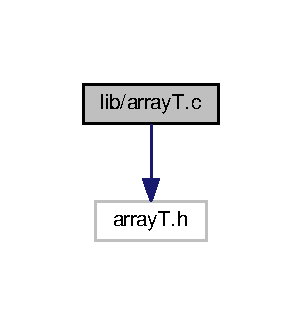
\includegraphics[width=145pt]{arrayT_8c__incl}
\end{center}
\end{figure}
\subsection*{Classes}
\begin{DoxyCompactItemize}
\item 
struct \hyperlink{structtagnum}{tagnum}
\item 
struct \hyperlink{structarraytagnum}{arraytagnum}
\end{DoxyCompactItemize}
\subsection*{Functions}
\begin{DoxyCompactItemize}
\item 
A\+T\+Num \hyperlink{arrayT_8c_a6eccd372126c735ddc91d972aa04e9fe}{insere\+\_\+tagnum} (A\+T\+Num a, T\+Num t)
\begin{DoxyCompactList}\small\item\em Insere um par Tag-\/\+Num no array. \end{DoxyCompactList}\item 
T\+Num \hyperlink{arrayT_8c_a0a2a4ce157589de008482e3e0993a11f}{inc\+T\+Num} (T\+Num pair)
\begin{DoxyCompactList}\small\item\em Incrementa o número de ocorrências da tag. \end{DoxyCompactList}\item 
T\+Num \hyperlink{arrayT_8c_a41dd540d9cf0d0fb33e3bd0b4492552e}{create\+\_\+tnum\+\_\+pair} (char $\ast$fst, int snd)
\begin{DoxyCompactList}\small\item\em Cria um par Tag-\/\+Num. \end{DoxyCompactList}\item 
void \hyperlink{arrayT_8c_abbc55eb3caa9e365739942bd9ff3d497}{set\+\_\+tag\+\_\+tnum} (T\+Num pair, char $\ast$str)
\begin{DoxyCompactList}\small\item\em Altera o campo \char`\"{}tag\char`\"{} de um T\+Num. \end{DoxyCompactList}\item 
void \hyperlink{arrayT_8c_acd4b96fdb4c967d3b5aff403fee3fe39}{set\+\_\+num\+\_\+tnum} (T\+Num pair, int num)
\begin{DoxyCompactList}\small\item\em Altera o campo \char`\"{}num\char`\"{} de um T\+Num. \end{DoxyCompactList}\item 
char $\ast$ \hyperlink{arrayT_8c_a99edf9d86c527b53b434e35f133350f5}{get\+\_\+tag\+\_\+tnum} (T\+Num pair)
\begin{DoxyCompactList}\small\item\em Retorna a string com o nome da tag. \end{DoxyCompactList}\item 
int \hyperlink{arrayT_8c_a5cbb235d67fbd34af6d26a9a414fba72}{get\+\_\+num\+\_\+tnum} (T\+Num pair)
\begin{DoxyCompactList}\small\item\em Retorna o número de ocorrências de uma tag. \end{DoxyCompactList}\item 
void \hyperlink{arrayT_8c_acd330c8b1e9f7a4456bc4ef307fa939b}{free\+\_\+tnum} (T\+Num pair)
\begin{DoxyCompactList}\small\item\em Liberta a memória alocada por um par Tag-\/\+Num. \end{DoxyCompactList}\item 
T\+Num \hyperlink{arrayT_8c_a8d50b369aff0c3800d385bae4048db03}{get\+\_\+atnum\+\_\+tnum} (A\+T\+Num pares, int index)
\begin{DoxyCompactList}\small\item\em Retorna um par Tag-\/\+Num de um determinado índice de um array de pares Tag-\/\+Num. \end{DoxyCompactList}\item 
long \hyperlink{arrayT_8c_a94e991303e5ad9c09f141a7ccf8651b0}{get\+\_\+atnum\+\_\+used} (A\+T\+Num a)
\begin{DoxyCompactList}\small\item\em Retorna o número de índices usados. \end{DoxyCompactList}\item 
long \hyperlink{arrayT_8c_ac819edb6d77158b271be466f4a9e7f0a}{get\+\_\+atnum\+\_\+size} (A\+T\+Num pares)
\begin{DoxyCompactList}\small\item\em Retorna o tamanho total do array. \end{DoxyCompactList}\item 
A\+T\+Num \hyperlink{arrayT_8c_a7cc1f39b6813c3343fd22f96203135e7}{init\+\_\+atnum} (long N)
\begin{DoxyCompactList}\small\item\em Cria um array de pares Tag-\/\+Num. \end{DoxyCompactList}\item 
void \hyperlink{arrayT_8c_a287a7386d14c8d4fb56a885fd1744f54}{bubble\+T\+Num\+Sort} (A\+T\+Num pares)
\begin{DoxyCompactList}\small\item\em Função que ordena por ordem decrescente do número de ocorrências os pares Tag-\/\+Num. \end{DoxyCompactList}\end{DoxyCompactItemize}


\subsection{Detailed Description}
Ficheiro que contém a implementação de um Array com uma \hyperlink{structtag}{tag(char$\ast$)} e o número de ocorrências. 



\subsection{Function Documentation}
\index{array\+T.\+c@{array\+T.\+c}!bubble\+T\+Num\+Sort@{bubble\+T\+Num\+Sort}}
\index{bubble\+T\+Num\+Sort@{bubble\+T\+Num\+Sort}!array\+T.\+c@{array\+T.\+c}}
\subsubsection[{\texorpdfstring{bubble\+T\+Num\+Sort(\+A\+T\+Num pares)}{bubbleTNumSort(ATNum pares)}}]{\setlength{\rightskip}{0pt plus 5cm}void bubble\+T\+Num\+Sort (
\begin{DoxyParamCaption}
\item[{A\+T\+Num}]{pares}
\end{DoxyParamCaption}
)}\hypertarget{arrayT_8c_a287a7386d14c8d4fb56a885fd1744f54}{}\label{arrayT_8c_a287a7386d14c8d4fb56a885fd1744f54}


Função que ordena por ordem decrescente do número de ocorrências os pares Tag-\/\+Num. 


\begin{DoxyParams}{Parameters}
{\em A\+T\+Num} & array de pares T\+Num. \\
\hline
\end{DoxyParams}
\index{array\+T.\+c@{array\+T.\+c}!create\+\_\+tnum\+\_\+pair@{create\+\_\+tnum\+\_\+pair}}
\index{create\+\_\+tnum\+\_\+pair@{create\+\_\+tnum\+\_\+pair}!array\+T.\+c@{array\+T.\+c}}
\subsubsection[{\texorpdfstring{create\+\_\+tnum\+\_\+pair(char $\ast$fst, int snd)}{create_tnum_pair(char *fst, int snd)}}]{\setlength{\rightskip}{0pt plus 5cm}T\+Num create\+\_\+tnum\+\_\+pair (
\begin{DoxyParamCaption}
\item[{char $\ast$}]{fst, }
\item[{int}]{snd}
\end{DoxyParamCaption}
)}\hypertarget{arrayT_8c_a41dd540d9cf0d0fb33e3bd0b4492552e}{}\label{arrayT_8c_a41dd540d9cf0d0fb33e3bd0b4492552e}


Cria um par Tag-\/\+Num. 


\begin{DoxyParams}{Parameters}
{\em char$\ast$} & string com o nome da tag. \\
\hline
{\em int} & número de ocorrências da tag. \\
\hline
\end{DoxyParams}
\begin{DoxyReturn}{Returns}
T\+Num par Tag-\/\+Num. 
\end{DoxyReturn}
\index{array\+T.\+c@{array\+T.\+c}!free\+\_\+tnum@{free\+\_\+tnum}}
\index{free\+\_\+tnum@{free\+\_\+tnum}!array\+T.\+c@{array\+T.\+c}}
\subsubsection[{\texorpdfstring{free\+\_\+tnum(\+T\+Num pair)}{free_tnum(TNum pair)}}]{\setlength{\rightskip}{0pt plus 5cm}void free\+\_\+tnum (
\begin{DoxyParamCaption}
\item[{T\+Num}]{pair}
\end{DoxyParamCaption}
)}\hypertarget{arrayT_8c_acd330c8b1e9f7a4456bc4ef307fa939b}{}\label{arrayT_8c_acd330c8b1e9f7a4456bc4ef307fa939b}


Liberta a memória alocada por um par Tag-\/\+Num. 


\begin{DoxyParams}{Parameters}
{\em T\+Num} & par Tag-\/\+Num. \\
\hline
\end{DoxyParams}
\index{array\+T.\+c@{array\+T.\+c}!get\+\_\+atnum\+\_\+size@{get\+\_\+atnum\+\_\+size}}
\index{get\+\_\+atnum\+\_\+size@{get\+\_\+atnum\+\_\+size}!array\+T.\+c@{array\+T.\+c}}
\subsubsection[{\texorpdfstring{get\+\_\+atnum\+\_\+size(\+A\+T\+Num pares)}{get_atnum_size(ATNum pares)}}]{\setlength{\rightskip}{0pt plus 5cm}long get\+\_\+atnum\+\_\+size (
\begin{DoxyParamCaption}
\item[{A\+T\+Num}]{pares}
\end{DoxyParamCaption}
)}\hypertarget{arrayT_8c_ac819edb6d77158b271be466f4a9e7f0a}{}\label{arrayT_8c_ac819edb6d77158b271be466f4a9e7f0a}


Retorna o tamanho total do array. 


\begin{DoxyParams}{Parameters}
{\em A\+T\+Num} & array de pares T\+Num. \\
\hline
\end{DoxyParams}
\begin{DoxyReturn}{Returns}
long tamanho total do array. 
\end{DoxyReturn}
\index{array\+T.\+c@{array\+T.\+c}!get\+\_\+atnum\+\_\+tnum@{get\+\_\+atnum\+\_\+tnum}}
\index{get\+\_\+atnum\+\_\+tnum@{get\+\_\+atnum\+\_\+tnum}!array\+T.\+c@{array\+T.\+c}}
\subsubsection[{\texorpdfstring{get\+\_\+atnum\+\_\+tnum(\+A\+T\+Num pares, int index)}{get_atnum_tnum(ATNum pares, int index)}}]{\setlength{\rightskip}{0pt plus 5cm}T\+Num get\+\_\+atnum\+\_\+tnum (
\begin{DoxyParamCaption}
\item[{A\+T\+Num}]{pares, }
\item[{int}]{index}
\end{DoxyParamCaption}
)}\hypertarget{arrayT_8c_a8d50b369aff0c3800d385bae4048db03}{}\label{arrayT_8c_a8d50b369aff0c3800d385bae4048db03}


Retorna um par Tag-\/\+Num de um determinado índice de um array de pares Tag-\/\+Num. 


\begin{DoxyParams}{Parameters}
{\em A\+T\+Num} & array de pares T\+Num. \\
\hline
{\em int} & índice. \\
\hline
\end{DoxyParams}
\begin{DoxyReturn}{Returns}
T\+Num par Tag-\/\+Num. 
\end{DoxyReturn}
\index{array\+T.\+c@{array\+T.\+c}!get\+\_\+atnum\+\_\+used@{get\+\_\+atnum\+\_\+used}}
\index{get\+\_\+atnum\+\_\+used@{get\+\_\+atnum\+\_\+used}!array\+T.\+c@{array\+T.\+c}}
\subsubsection[{\texorpdfstring{get\+\_\+atnum\+\_\+used(\+A\+T\+Num a)}{get_atnum_used(ATNum a)}}]{\setlength{\rightskip}{0pt plus 5cm}long get\+\_\+atnum\+\_\+used (
\begin{DoxyParamCaption}
\item[{A\+T\+Num}]{a}
\end{DoxyParamCaption}
)}\hypertarget{arrayT_8c_a94e991303e5ad9c09f141a7ccf8651b0}{}\label{arrayT_8c_a94e991303e5ad9c09f141a7ccf8651b0}


Retorna o número de índices usados. 


\begin{DoxyParams}{Parameters}
{\em A\+T\+Num} & array de pares T\+Num. \\
\hline
\end{DoxyParams}
\begin{DoxyReturn}{Returns}
int número de índices usados no array. 
\end{DoxyReturn}
\index{array\+T.\+c@{array\+T.\+c}!get\+\_\+num\+\_\+tnum@{get\+\_\+num\+\_\+tnum}}
\index{get\+\_\+num\+\_\+tnum@{get\+\_\+num\+\_\+tnum}!array\+T.\+c@{array\+T.\+c}}
\subsubsection[{\texorpdfstring{get\+\_\+num\+\_\+tnum(\+T\+Num pair)}{get_num_tnum(TNum pair)}}]{\setlength{\rightskip}{0pt plus 5cm}int get\+\_\+num\+\_\+tnum (
\begin{DoxyParamCaption}
\item[{T\+Num}]{pair}
\end{DoxyParamCaption}
)}\hypertarget{arrayT_8c_a5cbb235d67fbd34af6d26a9a414fba72}{}\label{arrayT_8c_a5cbb235d67fbd34af6d26a9a414fba72}


Retorna o número de ocorrências de uma tag. 


\begin{DoxyParams}{Parameters}
{\em T\+Num} & par Tag-\/\+Num. \\
\hline
\end{DoxyParams}
\begin{DoxyReturn}{Returns}
int número de ocrrências da tag. 
\end{DoxyReturn}
\index{array\+T.\+c@{array\+T.\+c}!get\+\_\+tag\+\_\+tnum@{get\+\_\+tag\+\_\+tnum}}
\index{get\+\_\+tag\+\_\+tnum@{get\+\_\+tag\+\_\+tnum}!array\+T.\+c@{array\+T.\+c}}
\subsubsection[{\texorpdfstring{get\+\_\+tag\+\_\+tnum(\+T\+Num pair)}{get_tag_tnum(TNum pair)}}]{\setlength{\rightskip}{0pt plus 5cm}char$\ast$ get\+\_\+tag\+\_\+tnum (
\begin{DoxyParamCaption}
\item[{T\+Num}]{pair}
\end{DoxyParamCaption}
)}\hypertarget{arrayT_8c_a99edf9d86c527b53b434e35f133350f5}{}\label{arrayT_8c_a99edf9d86c527b53b434e35f133350f5}


Retorna a string com o nome da tag. 


\begin{DoxyParams}{Parameters}
{\em T\+Num} & par Tag-\/\+Num. \\
\hline
\end{DoxyParams}
\begin{DoxyReturn}{Returns}
char$\ast$ string com o nome da tag. 
\end{DoxyReturn}
\index{array\+T.\+c@{array\+T.\+c}!inc\+T\+Num@{inc\+T\+Num}}
\index{inc\+T\+Num@{inc\+T\+Num}!array\+T.\+c@{array\+T.\+c}}
\subsubsection[{\texorpdfstring{inc\+T\+Num(\+T\+Num pair)}{incTNum(TNum pair)}}]{\setlength{\rightskip}{0pt plus 5cm}T\+Num inc\+T\+Num (
\begin{DoxyParamCaption}
\item[{T\+Num}]{pair}
\end{DoxyParamCaption}
)}\hypertarget{arrayT_8c_a0a2a4ce157589de008482e3e0993a11f}{}\label{arrayT_8c_a0a2a4ce157589de008482e3e0993a11f}


Incrementa o número de ocorrências da tag. 


\begin{DoxyParams}{Parameters}
{\em T\+Num} & par Tag-\/\+Num. \\
\hline
\end{DoxyParams}
\begin{DoxyReturn}{Returns}
A\+T\+Num array de pares. 
\end{DoxyReturn}
\index{array\+T.\+c@{array\+T.\+c}!init\+\_\+atnum@{init\+\_\+atnum}}
\index{init\+\_\+atnum@{init\+\_\+atnum}!array\+T.\+c@{array\+T.\+c}}
\subsubsection[{\texorpdfstring{init\+\_\+atnum(long N)}{init_atnum(long N)}}]{\setlength{\rightskip}{0pt plus 5cm}A\+T\+Num init\+\_\+atnum (
\begin{DoxyParamCaption}
\item[{long}]{N}
\end{DoxyParamCaption}
)}\hypertarget{arrayT_8c_a7cc1f39b6813c3343fd22f96203135e7}{}\label{arrayT_8c_a7cc1f39b6813c3343fd22f96203135e7}


Cria um array de pares Tag-\/\+Num. 


\begin{DoxyParams}{Parameters}
{\em long} & tamanho total (inicial) do aray. \\
\hline
\end{DoxyParams}
\begin{DoxyReturn}{Returns}
A\+T\+Num array de pares Tag-\/\+Num criado. 
\end{DoxyReturn}
\index{array\+T.\+c@{array\+T.\+c}!insere\+\_\+tagnum@{insere\+\_\+tagnum}}
\index{insere\+\_\+tagnum@{insere\+\_\+tagnum}!array\+T.\+c@{array\+T.\+c}}
\subsubsection[{\texorpdfstring{insere\+\_\+tagnum(\+A\+T\+Num a, T\+Num t)}{insere_tagnum(ATNum a, TNum t)}}]{\setlength{\rightskip}{0pt plus 5cm}A\+T\+Num insere\+\_\+tagnum (
\begin{DoxyParamCaption}
\item[{A\+T\+Num}]{a, }
\item[{T\+Num}]{t}
\end{DoxyParamCaption}
)}\hypertarget{arrayT_8c_a6eccd372126c735ddc91d972aa04e9fe}{}\label{arrayT_8c_a6eccd372126c735ddc91d972aa04e9fe}


Insere um par Tag-\/\+Num no array. 


\begin{DoxyParams}{Parameters}
{\em A\+Tnum} & array de pares Tag-\/\+Num. \\
\hline
{\em T\+Num} & par Tag-\/\+Num. \\
\hline
\end{DoxyParams}
\begin{DoxyReturn}{Returns}
A\+T\+Num array de pares. 
\end{DoxyReturn}
\index{array\+T.\+c@{array\+T.\+c}!set\+\_\+num\+\_\+tnum@{set\+\_\+num\+\_\+tnum}}
\index{set\+\_\+num\+\_\+tnum@{set\+\_\+num\+\_\+tnum}!array\+T.\+c@{array\+T.\+c}}
\subsubsection[{\texorpdfstring{set\+\_\+num\+\_\+tnum(\+T\+Num pair, int num)}{set_num_tnum(TNum pair, int num)}}]{\setlength{\rightskip}{0pt plus 5cm}void set\+\_\+num\+\_\+tnum (
\begin{DoxyParamCaption}
\item[{T\+Num}]{pair, }
\item[{int}]{num}
\end{DoxyParamCaption}
)}\hypertarget{arrayT_8c_acd4b96fdb4c967d3b5aff403fee3fe39}{}\label{arrayT_8c_acd4b96fdb4c967d3b5aff403fee3fe39}


Altera o campo \char`\"{}num\char`\"{} de um T\+Num. 


\begin{DoxyParams}{Parameters}
{\em T\+Num} & par Tag-\/\+Num. \\
\hline
{\em int} & número de ocorrências a colocar no par. \\
\hline
\end{DoxyParams}
\begin{DoxyReturn}{Returns}
A\+T\+Num array de pares. 
\end{DoxyReturn}
\index{array\+T.\+c@{array\+T.\+c}!set\+\_\+tag\+\_\+tnum@{set\+\_\+tag\+\_\+tnum}}
\index{set\+\_\+tag\+\_\+tnum@{set\+\_\+tag\+\_\+tnum}!array\+T.\+c@{array\+T.\+c}}
\subsubsection[{\texorpdfstring{set\+\_\+tag\+\_\+tnum(\+T\+Num pair, char $\ast$str)}{set_tag_tnum(TNum pair, char *str)}}]{\setlength{\rightskip}{0pt plus 5cm}void set\+\_\+tag\+\_\+tnum (
\begin{DoxyParamCaption}
\item[{T\+Num}]{pair, }
\item[{char $\ast$}]{str}
\end{DoxyParamCaption}
)}\hypertarget{arrayT_8c_abbc55eb3caa9e365739942bd9ff3d497}{}\label{arrayT_8c_abbc55eb3caa9e365739942bd9ff3d497}


Altera o campo \char`\"{}tag\char`\"{} de um T\+Num. 


\begin{DoxyParams}{Parameters}
{\em T\+Num} & par Tag-\/\+Num. \\
\hline
{\em char$\ast$} & string com o nome da tag. \\
\hline
\end{DoxyParams}
\begin{DoxyReturn}{Returns}
T\+Num par Tag-\/\+Num. 
\end{DoxyReturn}

\hypertarget{heap_8c}{}\section{lib/heap.c File Reference}
\label{heap_8c}\index{lib/heap.\+c@{lib/heap.\+c}}


Ficheiro que contém a implementação de Max Heap\textquotesingle{}s de Posts.  


{\ttfamily \#include \char`\"{}heap.\+h\char`\"{}}\\*
Include dependency graph for heap.\+c\+:
\nopagebreak
\begin{figure}[H]
\begin{center}
\leavevmode
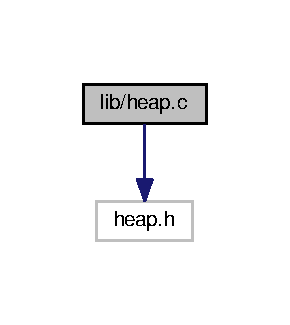
\includegraphics[width=139pt]{heap_8c__incl}
\end{center}
\end{figure}
\subsection*{Classes}
\begin{DoxyCompactItemize}
\item 
struct \hyperlink{structheap}{heap}
\end{DoxyCompactItemize}
\subsection*{Macros}
\begin{DoxyCompactItemize}
\item 
\#define {\bfseries P\+AI}(i)~(i-\/1)/2\hypertarget{heap_8c_a14497210befd92eb06223d770691914f}{}\label{heap_8c_a14497210befd92eb06223d770691914f}

\item 
\#define {\bfseries E\+S\+Q\+U\+E\+R\+DO}(i)~2$\ast$i + 1\hypertarget{heap_8c_aec0cd9b4eb09bfe7a565a67af16afe93}{}\label{heap_8c_aec0cd9b4eb09bfe7a565a67af16afe93}

\item 
\#define {\bfseries D\+I\+R\+E\+I\+TO}(i)~2$\ast$i + 2\hypertarget{heap_8c_ac6e409ddb66a55671170033763e3bb41}{}\label{heap_8c_ac6e409ddb66a55671170033763e3bb41}

\end{DoxyCompactItemize}
\subsection*{Functions}
\begin{DoxyCompactItemize}
\item 
int \hyperlink{heap_8c_a2c1c49ae1a90173c3552e091f075872f}{mais\+Recente} (Date date1, Date date2)
\begin{DoxyCompactList}\small\item\em Compara duas datas. \end{DoxyCompactList}\item 
static Heap \hyperlink{heap_8c_a63a74d52123275bd3abe9b01cecf3131}{swap} (Heap \hyperlink{structheap}{heap}, int n1, int n2)
\begin{DoxyCompactList}\small\item\em Troca dois elementos da heap. \end{DoxyCompactList}\item 
static Heap \hyperlink{heap_8c_a9206bc25fe50ab5a7e9980e10837f324}{bubble\+Down} (Heap \hyperlink{structheap}{heap}, int n, char ord)
\begin{DoxyCompactList}\small\item\em Realiza o bubble down da heap. \end{DoxyCompactList}\item 
static Heap \hyperlink{heap_8c_ae688b66c4e24bc6d8c0b2e0f5ec1414b}{bubble\+Up} (Heap \hyperlink{structheap}{heap}, int i, char ord)
\begin{DoxyCompactList}\small\item\em Realiza o bubble up da heap. \end{DoxyCompactList}\item 
Heap \hyperlink{heap_8c_abf46e093e8100cebe3aca6545aead1c5}{init\+Heap} ()
\begin{DoxyCompactList}\small\item\em Inicia uma nova heap de posts. \end{DoxyCompactList}\item 
Heap \hyperlink{heap_8c_a723709e7ce9f31c874a07eaf6b800db5}{init\+Heap\+Pal} (char $\ast$word)
\begin{DoxyCompactList}\small\item\em Inicia uma nova heap de posts que guarda adicionalmente uma dada palavra. \end{DoxyCompactList}\item 
char $\ast$ \hyperlink{heap_8c_ad750d8237bbcc3bad7b2183544f00f02}{get\+Heap\+Pal} (Heap h)
\begin{DoxyCompactList}\small\item\em Devolve a palavra guardada na heap. \end{DoxyCompactList}\item 
Heap \hyperlink{heap_8c_a57b1aa828dd4a3a09eecdbe2c2a014d4}{heap\+\_\+push} (Heap \hyperlink{structheap}{heap}, Post \hyperlink{structpost}{post}, char ord)
\begin{DoxyCompactList}\small\item\em Insere um post na heap tendo como referência o parâmetro da ordenação. \end{DoxyCompactList}\item 
Post \hyperlink{heap_8c_a9116376c941be4c76d96916042f4d1e5}{heap\+\_\+pop} (Heap \hyperlink{structheap}{heap}, char ord)
\begin{DoxyCompactList}\small\item\em Retorna o \char`\"{}maior\char`\"{} post segundo a ordenação dada. \end{DoxyCompactList}\item 
int \hyperlink{heap_8c_a09a4c1174fbd9f4164ae68d20cea24b5}{heap\+\_\+count} (Heap \hyperlink{structheap}{heap})
\begin{DoxyCompactList}\small\item\em Retorna o número de posts que uma dada heap contém. \end{DoxyCompactList}\item 
int \hyperlink{heap_8c_a1128d5e75bb67d2d8b5f35574295fb62}{cont\+\_\+\+RP} (Heap \hyperlink{structheap}{heap})
\begin{DoxyCompactList}\small\item\em Retorna o número de perguntas e respostas que uma dada heap de posts contém. \end{DoxyCompactList}\item 
Post \hyperlink{heap_8c_a952e32177af090cd2480a3183b242155}{get\+IndP} (Heap h, int i)
\begin{DoxyCompactList}\small\item\em Retorna o Post que se encontrada num indice i de uma dada heap. \end{DoxyCompactList}\item 
void \hyperlink{heap_8c_a085d0249b7c1c9e5b2de6333b9fdc92b}{heap\+\_\+free} (Heap \hyperlink{structheap}{heap})
\begin{DoxyCompactList}\small\item\em Liberta a memória alocada por uma Heap. \end{DoxyCompactList}\item 
void {\bfseries heap\+Pal\+\_\+free} (Heap \hyperlink{structheap}{heap})\hypertarget{heap_8c_a2e2677ca709a7d6cae69c2cfc211d998}{}\label{heap_8c_a2e2677ca709a7d6cae69c2cfc211d998}

\end{DoxyCompactItemize}


\subsection{Detailed Description}
Ficheiro que contém a implementação de Max Heap\textquotesingle{}s de Posts. 



\subsection{Function Documentation}
\index{heap.\+c@{heap.\+c}!bubble\+Down@{bubble\+Down}}
\index{bubble\+Down@{bubble\+Down}!heap.\+c@{heap.\+c}}
\subsubsection[{\texorpdfstring{bubble\+Down(\+Heap heap, int n, char ord)}{bubbleDown(Heap heap, int n, char ord)}}]{\setlength{\rightskip}{0pt plus 5cm}static Heap bubble\+Down (
\begin{DoxyParamCaption}
\item[{Heap}]{heap, }
\item[{int}]{n, }
\item[{char}]{ord}
\end{DoxyParamCaption}
)\hspace{0.3cm}{\ttfamily [static]}}\hypertarget{heap_8c_a9206bc25fe50ab5a7e9980e10837f324}{}\label{heap_8c_a9206bc25fe50ab5a7e9980e10837f324}


Realiza o bubble down da heap. 


\begin{DoxyParams}{Parameters}
{\em Heap} & heap a alterar. \\
\hline
\end{DoxyParams}
\begin{DoxyReturn}{Returns}
Heap alterada. 
\end{DoxyReturn}
\index{heap.\+c@{heap.\+c}!bubble\+Up@{bubble\+Up}}
\index{bubble\+Up@{bubble\+Up}!heap.\+c@{heap.\+c}}
\subsubsection[{\texorpdfstring{bubble\+Up(\+Heap heap, int i, char ord)}{bubbleUp(Heap heap, int i, char ord)}}]{\setlength{\rightskip}{0pt plus 5cm}static Heap bubble\+Up (
\begin{DoxyParamCaption}
\item[{Heap}]{heap, }
\item[{int}]{i, }
\item[{char}]{ord}
\end{DoxyParamCaption}
)\hspace{0.3cm}{\ttfamily [static]}}\hypertarget{heap_8c_ae688b66c4e24bc6d8c0b2e0f5ec1414b}{}\label{heap_8c_ae688b66c4e24bc6d8c0b2e0f5ec1414b}


Realiza o bubble up da heap. 


\begin{DoxyParams}{Parameters}
{\em Heap} & heap a alterar. \\
\hline
\end{DoxyParams}
\begin{DoxyReturn}{Returns}
Heap alterada. 
\end{DoxyReturn}
\index{heap.\+c@{heap.\+c}!cont\+\_\+\+RP@{cont\+\_\+\+RP}}
\index{cont\+\_\+\+RP@{cont\+\_\+\+RP}!heap.\+c@{heap.\+c}}
\subsubsection[{\texorpdfstring{cont\+\_\+\+R\+P(\+Heap heap)}{cont_RP(Heap heap)}}]{\setlength{\rightskip}{0pt plus 5cm}int cont\+\_\+\+RP (
\begin{DoxyParamCaption}
\item[{Heap}]{heap}
\end{DoxyParamCaption}
)}\hypertarget{heap_8c_a1128d5e75bb67d2d8b5f35574295fb62}{}\label{heap_8c_a1128d5e75bb67d2d8b5f35574295fb62}


Retorna o número de perguntas e respostas que uma dada heap de posts contém. 


\begin{DoxyParams}{Parameters}
{\em Heap} & heap. \\
\hline
\end{DoxyParams}
\begin{DoxyReturn}{Returns}
int número de posts na heap. 
\end{DoxyReturn}
\index{heap.\+c@{heap.\+c}!get\+Heap\+Pal@{get\+Heap\+Pal}}
\index{get\+Heap\+Pal@{get\+Heap\+Pal}!heap.\+c@{heap.\+c}}
\subsubsection[{\texorpdfstring{get\+Heap\+Pal(\+Heap h)}{getHeapPal(Heap h)}}]{\setlength{\rightskip}{0pt plus 5cm}char$\ast$ get\+Heap\+Pal (
\begin{DoxyParamCaption}
\item[{Heap}]{h}
\end{DoxyParamCaption}
)}\hypertarget{heap_8c_ad750d8237bbcc3bad7b2183544f00f02}{}\label{heap_8c_ad750d8237bbcc3bad7b2183544f00f02}


Devolve a palavra guardada na heap. 


\begin{DoxyParams}{Parameters}
{\em Heap} & heap. \\
\hline
\end{DoxyParams}
\begin{DoxyReturn}{Returns}
char$\ast$ palavra. 
\end{DoxyReturn}
\index{heap.\+c@{heap.\+c}!get\+IndP@{get\+IndP}}
\index{get\+IndP@{get\+IndP}!heap.\+c@{heap.\+c}}
\subsubsection[{\texorpdfstring{get\+Ind\+P(\+Heap h, int i)}{getIndP(Heap h, int i)}}]{\setlength{\rightskip}{0pt plus 5cm}Post get\+IndP (
\begin{DoxyParamCaption}
\item[{Heap}]{h, }
\item[{int}]{i}
\end{DoxyParamCaption}
)}\hypertarget{heap_8c_a952e32177af090cd2480a3183b242155}{}\label{heap_8c_a952e32177af090cd2480a3183b242155}


Retorna o Post que se encontrada num indice i de uma dada heap. 


\begin{DoxyParams}{Parameters}
{\em Heap} & heap. \\
\hline
{\em int} & i. return Post na posição i da heap. \\
\hline
\end{DoxyParams}
\index{heap.\+c@{heap.\+c}!heap\+\_\+count@{heap\+\_\+count}}
\index{heap\+\_\+count@{heap\+\_\+count}!heap.\+c@{heap.\+c}}
\subsubsection[{\texorpdfstring{heap\+\_\+count(\+Heap heap)}{heap_count(Heap heap)}}]{\setlength{\rightskip}{0pt plus 5cm}int heap\+\_\+count (
\begin{DoxyParamCaption}
\item[{Heap}]{heap}
\end{DoxyParamCaption}
)}\hypertarget{heap_8c_a09a4c1174fbd9f4164ae68d20cea24b5}{}\label{heap_8c_a09a4c1174fbd9f4164ae68d20cea24b5}


Retorna o número de posts que uma dada heap contém. 


\begin{DoxyParams}{Parameters}
{\em Heap} & heap. \\
\hline
\end{DoxyParams}
\begin{DoxyReturn}{Returns}
int número de Posts na heap. 
\end{DoxyReturn}
\index{heap.\+c@{heap.\+c}!heap\+\_\+free@{heap\+\_\+free}}
\index{heap\+\_\+free@{heap\+\_\+free}!heap.\+c@{heap.\+c}}
\subsubsection[{\texorpdfstring{heap\+\_\+free(\+Heap heap)}{heap_free(Heap heap)}}]{\setlength{\rightskip}{0pt plus 5cm}void heap\+\_\+free (
\begin{DoxyParamCaption}
\item[{Heap}]{heap}
\end{DoxyParamCaption}
)}\hypertarget{heap_8c_a085d0249b7c1c9e5b2de6333b9fdc92b}{}\label{heap_8c_a085d0249b7c1c9e5b2de6333b9fdc92b}


Liberta a memória alocada por uma Heap. 


\begin{DoxyParams}{Parameters}
{\em void$\ast$} & apontador para a heap a limpar da memória. \\
\hline
\end{DoxyParams}
\index{heap.\+c@{heap.\+c}!heap\+\_\+pop@{heap\+\_\+pop}}
\index{heap\+\_\+pop@{heap\+\_\+pop}!heap.\+c@{heap.\+c}}
\subsubsection[{\texorpdfstring{heap\+\_\+pop(\+Heap heap, char ord)}{heap_pop(Heap heap, char ord)}}]{\setlength{\rightskip}{0pt plus 5cm}Post heap\+\_\+pop (
\begin{DoxyParamCaption}
\item[{Heap}]{heap, }
\item[{char}]{ord}
\end{DoxyParamCaption}
)}\hypertarget{heap_8c_a9116376c941be4c76d96916042f4d1e5}{}\label{heap_8c_a9116376c941be4c76d96916042f4d1e5}


Retorna o \char`\"{}maior\char`\"{} post segundo a ordenação dada. 


\begin{DoxyParams}{Parameters}
{\em Heap} & heap de todos os posts. \\
\hline
{\em char} & ordenação segundo a qual a Heap se ordena. \\
\hline
\end{DoxyParams}
\begin{DoxyReturn}{Returns}
Post removido. 
\end{DoxyReturn}
\index{heap.\+c@{heap.\+c}!heap\+\_\+push@{heap\+\_\+push}}
\index{heap\+\_\+push@{heap\+\_\+push}!heap.\+c@{heap.\+c}}
\subsubsection[{\texorpdfstring{heap\+\_\+push(\+Heap heap, Post post, char ord)}{heap_push(Heap heap, Post post, char ord)}}]{\setlength{\rightskip}{0pt plus 5cm}Heap heap\+\_\+push (
\begin{DoxyParamCaption}
\item[{Heap}]{heap, }
\item[{Post}]{post, }
\item[{char}]{ord}
\end{DoxyParamCaption}
)}\hypertarget{heap_8c_a57b1aa828dd4a3a09eecdbe2c2a014d4}{}\label{heap_8c_a57b1aa828dd4a3a09eecdbe2c2a014d4}


Insere um post na heap tendo como referência o parâmetro da ordenação. 


\begin{DoxyParams}{Parameters}
{\em Heap} & heap. \\
\hline
{\em Post} & post. \\
\hline
{\em char} & caracter que determina a ordenação (D-\/\+Data do post, S-\/\+Score do post, R-\/\+Número de respostas do post, M-\/\+Média ponderada da classificação do post). \\
\hline
\end{DoxyParams}
\begin{DoxyReturn}{Returns}
Heap com o novo Post adicionado. 
\end{DoxyReturn}
\index{heap.\+c@{heap.\+c}!init\+Heap@{init\+Heap}}
\index{init\+Heap@{init\+Heap}!heap.\+c@{heap.\+c}}
\subsubsection[{\texorpdfstring{init\+Heap()}{initHeap()}}]{\setlength{\rightskip}{0pt plus 5cm}Heap init\+Heap (
\begin{DoxyParamCaption}
{}
\end{DoxyParamCaption}
)}\hypertarget{heap_8c_abf46e093e8100cebe3aca6545aead1c5}{}\label{heap_8c_abf46e093e8100cebe3aca6545aead1c5}


Inicia uma nova heap de posts. 

\begin{DoxyReturn}{Returns}
Heap inicializada. 
\end{DoxyReturn}
\index{heap.\+c@{heap.\+c}!init\+Heap\+Pal@{init\+Heap\+Pal}}
\index{init\+Heap\+Pal@{init\+Heap\+Pal}!heap.\+c@{heap.\+c}}
\subsubsection[{\texorpdfstring{init\+Heap\+Pal(char $\ast$word)}{initHeapPal(char *word)}}]{\setlength{\rightskip}{0pt plus 5cm}Heap init\+Heap\+Pal (
\begin{DoxyParamCaption}
\item[{char $\ast$}]{word}
\end{DoxyParamCaption}
)}\hypertarget{heap_8c_a723709e7ce9f31c874a07eaf6b800db5}{}\label{heap_8c_a723709e7ce9f31c874a07eaf6b800db5}


Inicia uma nova heap de posts que guarda adicionalmente uma dada palavra. 


\begin{DoxyParams}{Parameters}
{\em char$\ast$} & palavra. \\
\hline
\end{DoxyParams}
\begin{DoxyReturn}{Returns}
Heap inicializada. 
\end{DoxyReturn}
\index{heap.\+c@{heap.\+c}!mais\+Recente@{mais\+Recente}}
\index{mais\+Recente@{mais\+Recente}!heap.\+c@{heap.\+c}}
\subsubsection[{\texorpdfstring{mais\+Recente(\+Date date1, Date date2)}{maisRecente(Date date1, Date date2)}}]{\setlength{\rightskip}{0pt plus 5cm}int mais\+Recente (
\begin{DoxyParamCaption}
\item[{Date}]{date1, }
\item[{Date}]{date2}
\end{DoxyParamCaption}
)}\hypertarget{heap_8c_a2c1c49ae1a90173c3552e091f075872f}{}\label{heap_8c_a2c1c49ae1a90173c3552e091f075872f}


Compara duas datas. 


\begin{DoxyParams}{Parameters}
{\em Date} & data1. \\
\hline
{\em Date} & data2. \\
\hline
\end{DoxyParams}
\begin{DoxyReturn}{Returns}
int resultado da comparação (-\/1 se data1 for a mais recente, 1 se data2 for a mais recente ou 0 se forem iguais). 
\end{DoxyReturn}
\index{heap.\+c@{heap.\+c}!swap@{swap}}
\index{swap@{swap}!heap.\+c@{heap.\+c}}
\subsubsection[{\texorpdfstring{swap(\+Heap heap, int n1, int n2)}{swap(Heap heap, int n1, int n2)}}]{\setlength{\rightskip}{0pt plus 5cm}static Heap swap (
\begin{DoxyParamCaption}
\item[{Heap}]{heap, }
\item[{int}]{n1, }
\item[{int}]{n2}
\end{DoxyParamCaption}
)\hspace{0.3cm}{\ttfamily [static]}}\hypertarget{heap_8c_a63a74d52123275bd3abe9b01cecf3131}{}\label{heap_8c_a63a74d52123275bd3abe9b01cecf3131}


Troca dois elementos da heap. 


\begin{DoxyParams}{Parameters}
{\em int} & posição do primeiro elemento. \\
\hline
{\em int} & posição do segundo elemento. \\
\hline
\end{DoxyParams}
\begin{DoxyReturn}{Returns}
Heap alterada. 
\end{DoxyReturn}

\hypertarget{heapU_8c}{}\section{lib/heapU.c File Reference}
\label{heapU_8c}\index{lib/heap\+U.\+c@{lib/heap\+U.\+c}}


Ficheiro que contém a implementação de Max Heap\textquotesingle{}s.  


{\ttfamily \#include \char`\"{}heap\+U.\+h\char`\"{}}\\*
Include dependency graph for heap\+U.\+c\+:
\nopagebreak
\begin{figure}[H]
\begin{center}
\leavevmode
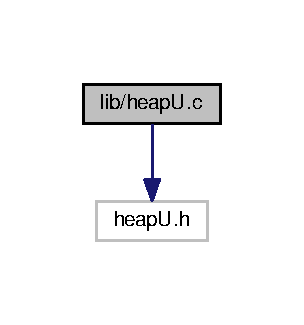
\includegraphics[width=146pt]{heapU_8c__incl}
\end{center}
\end{figure}
\subsection*{Classes}
\begin{DoxyCompactItemize}
\item 
struct \hyperlink{structheapu}{heapu}
\end{DoxyCompactItemize}
\subsection*{Macros}
\begin{DoxyCompactItemize}
\item 
\#define {\bfseries P\+AI}(i)~(i-\/1)/2\hypertarget{heapU_8c_a14497210befd92eb06223d770691914f}{}\label{heapU_8c_a14497210befd92eb06223d770691914f}

\item 
\#define {\bfseries E\+S\+Q\+U\+E\+R\+DO}(i)~2$\ast$i + 1\hypertarget{heapU_8c_aec0cd9b4eb09bfe7a565a67af16afe93}{}\label{heapU_8c_aec0cd9b4eb09bfe7a565a67af16afe93}

\item 
\#define {\bfseries D\+I\+R\+E\+I\+TO}(i)~2$\ast$i + 2\hypertarget{heapU_8c_ac6e409ddb66a55671170033763e3bb41}{}\label{heapU_8c_ac6e409ddb66a55671170033763e3bb41}

\end{DoxyCompactItemize}
\subsection*{Functions}
\begin{DoxyCompactItemize}
\item 
static void \hyperlink{heapU_8c_ae5951c47c7821b6a4952d56c5961f20a}{swapU} (HeapU \hyperlink{structheap}{heap}, int n1, int n2)
\begin{DoxyCompactList}\small\item\em Troca dois elementos da heap. \end{DoxyCompactList}\item 
static HeapU \hyperlink{heapU_8c_acd15aceb37c9c83fc919e6073ee0246f}{bubble\+DownU} (HeapU \hyperlink{structheap}{heap})
\begin{DoxyCompactList}\small\item\em Realiza o bubble down da Heap. \end{DoxyCompactList}\item 
static HeapU \hyperlink{heapU_8c_a3696fda6ee2450ff9a0ce984190c6c08}{bubble\+UpU} (HeapU \hyperlink{structheap}{heap})
\begin{DoxyCompactList}\small\item\em Realiza o bubble up da heap. \end{DoxyCompactList}\item 
HeapU \hyperlink{heapU_8c_a71e13067d181115791873282b7d4566d}{init\+HeapU} ()
\begin{DoxyCompactList}\small\item\em Inicia uma nova Heap. \end{DoxyCompactList}\item 
HeapU \hyperlink{heapU_8c_ad48877be615e59513222ebc1e37ce60c}{heap\+\_\+pushU} (HeapU \hyperlink{structheap}{heap}, long id, long qnt)
\begin{DoxyCompactList}\small\item\em Insere na Heap tendo como referência a quantidade. \end{DoxyCompactList}\item 
long \hyperlink{heapU_8c_a17a5145c43ad902b976f7b7bb41316ff}{heap\+\_\+popU} (HeapU \hyperlink{structheap}{heap})
\begin{DoxyCompactList}\small\item\em Retorna o maior elemento da Heap. \end{DoxyCompactList}\item 
int \hyperlink{heapU_8c_ae66235cc59d2729360f325539e919f70}{heap\+\_\+countU} (HeapU \hyperlink{structheap}{heap})
\begin{DoxyCompactList}\small\item\em Retorna o número de elementos de uma Heap. \end{DoxyCompactList}\item 
void \hyperlink{heapU_8c_a0fd1f3ded75be8fd561d8b2ee7434fb0}{heap\+\_\+freeU} (HeapU \hyperlink{structheap}{heap})
\begin{DoxyCompactList}\small\item\em Liberta a memória alocada por uma HeapU. \end{DoxyCompactList}\end{DoxyCompactItemize}


\subsection{Detailed Description}
Ficheiro que contém a implementação de Max Heap\textquotesingle{}s. 



\subsection{Function Documentation}
\index{heap\+U.\+c@{heap\+U.\+c}!bubble\+DownU@{bubble\+DownU}}
\index{bubble\+DownU@{bubble\+DownU}!heap\+U.\+c@{heap\+U.\+c}}
\subsubsection[{\texorpdfstring{bubble\+Down\+U(\+Heap\+U heap)}{bubbleDownU(HeapU heap)}}]{\setlength{\rightskip}{0pt plus 5cm}static HeapU bubble\+DownU (
\begin{DoxyParamCaption}
\item[{HeapU}]{heap}
\end{DoxyParamCaption}
)\hspace{0.3cm}{\ttfamily [static]}}\hypertarget{heapU_8c_acd15aceb37c9c83fc919e6073ee0246f}{}\label{heapU_8c_acd15aceb37c9c83fc919e6073ee0246f}


Realiza o bubble down da Heap. 


\begin{DoxyParams}{Parameters}
{\em HeapU} & heap a alterar. \\
\hline
\end{DoxyParams}
\begin{DoxyReturn}{Returns}
HeapU alterada. 
\end{DoxyReturn}
\index{heap\+U.\+c@{heap\+U.\+c}!bubble\+UpU@{bubble\+UpU}}
\index{bubble\+UpU@{bubble\+UpU}!heap\+U.\+c@{heap\+U.\+c}}
\subsubsection[{\texorpdfstring{bubble\+Up\+U(\+Heap\+U heap)}{bubbleUpU(HeapU heap)}}]{\setlength{\rightskip}{0pt plus 5cm}static HeapU bubble\+UpU (
\begin{DoxyParamCaption}
\item[{HeapU}]{heap}
\end{DoxyParamCaption}
)\hspace{0.3cm}{\ttfamily [static]}}\hypertarget{heapU_8c_a3696fda6ee2450ff9a0ce984190c6c08}{}\label{heapU_8c_a3696fda6ee2450ff9a0ce984190c6c08}


Realiza o bubble up da heap. 


\begin{DoxyParams}{Parameters}
{\em HeapU} & heap a alterar. \\
\hline
\end{DoxyParams}
\begin{DoxyReturn}{Returns}
HeapU alterada. 
\end{DoxyReturn}
\index{heap\+U.\+c@{heap\+U.\+c}!heap\+\_\+countU@{heap\+\_\+countU}}
\index{heap\+\_\+countU@{heap\+\_\+countU}!heap\+U.\+c@{heap\+U.\+c}}
\subsubsection[{\texorpdfstring{heap\+\_\+count\+U(\+Heap\+U heap)}{heap_countU(HeapU heap)}}]{\setlength{\rightskip}{0pt plus 5cm}int heap\+\_\+countU (
\begin{DoxyParamCaption}
\item[{HeapU}]{heap}
\end{DoxyParamCaption}
)}\hypertarget{heapU_8c_ae66235cc59d2729360f325539e919f70}{}\label{heapU_8c_ae66235cc59d2729360f325539e919f70}


Retorna o número de elementos de uma Heap. 


\begin{DoxyParams}{Parameters}
{\em HeapU} & heap. \\
\hline
\end{DoxyParams}
\begin{DoxyReturn}{Returns}
Número de elementos da heap. 
\end{DoxyReturn}
\index{heap\+U.\+c@{heap\+U.\+c}!heap\+\_\+freeU@{heap\+\_\+freeU}}
\index{heap\+\_\+freeU@{heap\+\_\+freeU}!heap\+U.\+c@{heap\+U.\+c}}
\subsubsection[{\texorpdfstring{heap\+\_\+free\+U(\+Heap\+U heap)}{heap_freeU(HeapU heap)}}]{\setlength{\rightskip}{0pt plus 5cm}void heap\+\_\+freeU (
\begin{DoxyParamCaption}
\item[{HeapU}]{heap}
\end{DoxyParamCaption}
)}\hypertarget{heapU_8c_a0fd1f3ded75be8fd561d8b2ee7434fb0}{}\label{heapU_8c_a0fd1f3ded75be8fd561d8b2ee7434fb0}


Liberta a memória alocada por uma HeapU. 


\begin{DoxyParams}{Parameters}
{\em void$\ast$} & apontador para a HeapU a limpar da memória. \\
\hline
\end{DoxyParams}
\index{heap\+U.\+c@{heap\+U.\+c}!heap\+\_\+popU@{heap\+\_\+popU}}
\index{heap\+\_\+popU@{heap\+\_\+popU}!heap\+U.\+c@{heap\+U.\+c}}
\subsubsection[{\texorpdfstring{heap\+\_\+pop\+U(\+Heap\+U heap)}{heap_popU(HeapU heap)}}]{\setlength{\rightskip}{0pt plus 5cm}long heap\+\_\+popU (
\begin{DoxyParamCaption}
\item[{HeapU}]{heap}
\end{DoxyParamCaption}
)}\hypertarget{heapU_8c_a17a5145c43ad902b976f7b7bb41316ff}{}\label{heapU_8c_a17a5145c43ad902b976f7b7bb41316ff}


Retorna o maior elemento da Heap. 


\begin{DoxyParams}{Parameters}
{\em HeapU} & da qual se retira o elemento. \\
\hline
\end{DoxyParams}
\begin{DoxyReturn}{Returns}
Id do elemento removido. 
\end{DoxyReturn}
\index{heap\+U.\+c@{heap\+U.\+c}!heap\+\_\+pushU@{heap\+\_\+pushU}}
\index{heap\+\_\+pushU@{heap\+\_\+pushU}!heap\+U.\+c@{heap\+U.\+c}}
\subsubsection[{\texorpdfstring{heap\+\_\+push\+U(\+Heap\+U heap, long id, long qnt)}{heap_pushU(HeapU heap, long id, long qnt)}}]{\setlength{\rightskip}{0pt plus 5cm}HeapU heap\+\_\+pushU (
\begin{DoxyParamCaption}
\item[{HeapU}]{heap, }
\item[{long}]{id, }
\item[{long}]{qnt}
\end{DoxyParamCaption}
)}\hypertarget{heapU_8c_ad48877be615e59513222ebc1e37ce60c}{}\label{heapU_8c_ad48877be615e59513222ebc1e37ce60c}


Insere na Heap tendo como referência a quantidade. 


\begin{DoxyParams}{Parameters}
{\em HeapU} & onde se insere. \\
\hline
{\em long} & id do elemento. \\
\hline
{\em long} & quantidade do elemento. \\
\hline
\end{DoxyParams}
\begin{DoxyReturn}{Returns}
HeapU com o novo elemento adicionado. 
\end{DoxyReturn}
\index{heap\+U.\+c@{heap\+U.\+c}!init\+HeapU@{init\+HeapU}}
\index{init\+HeapU@{init\+HeapU}!heap\+U.\+c@{heap\+U.\+c}}
\subsubsection[{\texorpdfstring{init\+Heap\+U()}{initHeapU()}}]{\setlength{\rightskip}{0pt plus 5cm}HeapU init\+HeapU (
\begin{DoxyParamCaption}
{}
\end{DoxyParamCaption}
)}\hypertarget{heapU_8c_a71e13067d181115791873282b7d4566d}{}\label{heapU_8c_a71e13067d181115791873282b7d4566d}


Inicia uma nova Heap. 

\begin{DoxyReturn}{Returns}
Nova HeapU nula. 
\end{DoxyReturn}
\index{heap\+U.\+c@{heap\+U.\+c}!swapU@{swapU}}
\index{swapU@{swapU}!heap\+U.\+c@{heap\+U.\+c}}
\subsubsection[{\texorpdfstring{swap\+U(\+Heap\+U heap, int n1, int n2)}{swapU(HeapU heap, int n1, int n2)}}]{\setlength{\rightskip}{0pt plus 5cm}static void swapU (
\begin{DoxyParamCaption}
\item[{HeapU}]{heap, }
\item[{int}]{n1, }
\item[{int}]{n2}
\end{DoxyParamCaption}
)\hspace{0.3cm}{\ttfamily [static]}}\hypertarget{heapU_8c_ae5951c47c7821b6a4952d56c5961f20a}{}\label{heapU_8c_ae5951c47c7821b6a4952d56c5961f20a}


Troca dois elementos da heap. 


\begin{DoxyParams}{Parameters}
{\em int} & posição do primeiro elemento. \\
\hline
{\em int} & posição do segundo elemento. \\
\hline
\end{DoxyParams}
\begin{DoxyReturn}{Returns}
HeapU alterada. 
\end{DoxyReturn}

\hypertarget{key_8c}{}\section{lib/key.c File Reference}
\label{key_8c}\index{lib/key.\+c@{lib/key.\+c}}


Ficheiro que contem a implementação de Keys. Uma Key é um apontador para um long.  


{\ttfamily \#include \char`\"{}key.\+h\char`\"{}}\\*
{\ttfamily \#include $<$stdlib.\+h$>$}\\*
Include dependency graph for key.\+c\+:
\nopagebreak
\begin{figure}[H]
\begin{center}
\leavevmode
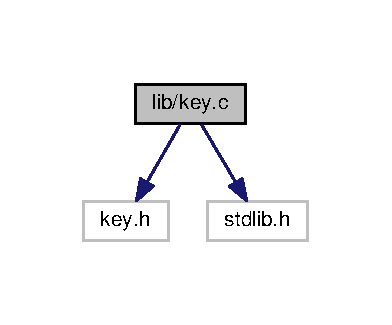
\includegraphics[width=188pt]{key_8c__incl}
\end{center}
\end{figure}
\subsection*{Classes}
\begin{DoxyCompactItemize}
\item 
struct \hyperlink{structkey}{key}
\end{DoxyCompactItemize}
\subsection*{Functions}
\begin{DoxyCompactItemize}
\item 
Key \hyperlink{key_8c_a98312906fb7539d5686b6ed4da8e4a83}{create\+Key} (long \hyperlink{structkey}{key})
\begin{DoxyCompactList}\small\item\em Converte um long numa Key. \end{DoxyCompactList}\item 
long \hyperlink{key_8c_aafa85a69939ac8b8cd9aba6246792345}{get\+Key} (Key k)
\begin{DoxyCompactList}\small\item\em Converte uma Key num long. \end{DoxyCompactList}\item 
void \hyperlink{key_8c_a5e45aa2012aec92f703a59dde97ba4b9}{freekey} (Key k)
\begin{DoxyCompactList}\small\item\em Liberta a memória alocada por uma Key. \end{DoxyCompactList}\end{DoxyCompactItemize}


\subsection{Detailed Description}
Ficheiro que contem a implementação de Keys. Uma Key é um apontador para um long. 



\subsection{Function Documentation}
\index{key.\+c@{key.\+c}!create\+Key@{create\+Key}}
\index{create\+Key@{create\+Key}!key.\+c@{key.\+c}}
\subsubsection[{\texorpdfstring{create\+Key(long key)}{createKey(long key)}}]{\setlength{\rightskip}{0pt plus 5cm}Key create\+Key (
\begin{DoxyParamCaption}
\item[{long}]{key}
\end{DoxyParamCaption}
)}\hypertarget{key_8c_a98312906fb7539d5686b6ed4da8e4a83}{}\label{key_8c_a98312906fb7539d5686b6ed4da8e4a83}


Converte um long numa Key. 


\begin{DoxyParams}{Parameters}
{\em long} & a ser convertido. \\
\hline
\end{DoxyParams}
\begin{DoxyReturn}{Returns}
Key criada. 
\end{DoxyReturn}
\index{key.\+c@{key.\+c}!freekey@{freekey}}
\index{freekey@{freekey}!key.\+c@{key.\+c}}
\subsubsection[{\texorpdfstring{freekey(\+Key k)}{freekey(Key k)}}]{\setlength{\rightskip}{0pt plus 5cm}void freekey (
\begin{DoxyParamCaption}
\item[{Key}]{k}
\end{DoxyParamCaption}
)}\hypertarget{key_8c_a5e45aa2012aec92f703a59dde97ba4b9}{}\label{key_8c_a5e45aa2012aec92f703a59dde97ba4b9}


Liberta a memória alocada por uma Key. 


\begin{DoxyParams}{Parameters}
{\em Key} & a ser libertada. \\
\hline
\end{DoxyParams}
\index{key.\+c@{key.\+c}!get\+Key@{get\+Key}}
\index{get\+Key@{get\+Key}!key.\+c@{key.\+c}}
\subsubsection[{\texorpdfstring{get\+Key(\+Key k)}{getKey(Key k)}}]{\setlength{\rightskip}{0pt plus 5cm}long get\+Key (
\begin{DoxyParamCaption}
\item[{Key}]{k}
\end{DoxyParamCaption}
)}\hypertarget{key_8c_aafa85a69939ac8b8cd9aba6246792345}{}\label{key_8c_aafa85a69939ac8b8cd9aba6246792345}


Converte uma Key num long. 


\begin{DoxyParams}{Parameters}
{\em Key} & a ser convertida. \\
\hline
\end{DoxyParams}
\begin{DoxyReturn}{Returns}
long. 
\end{DoxyReturn}

\hypertarget{mypost_8c}{}\section{lib/mypost.c File Reference}
\label{mypost_8c}\index{lib/mypost.\+c@{lib/mypost.\+c}}


Ficheiro que contém a implementação de Posts.  


{\ttfamily \#include \char`\"{}mypost.\+h\char`\"{}}\\*
Include dependency graph for mypost.\+c\+:
\nopagebreak
\begin{figure}[H]
\begin{center}
\leavevmode
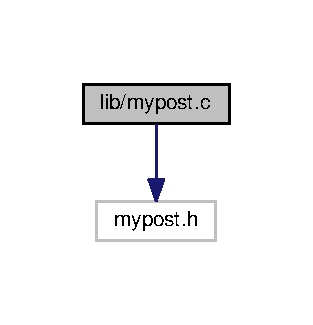
\includegraphics[width=150pt]{mypost_8c__incl}
\end{center}
\end{figure}
\subsection*{Classes}
\begin{DoxyCompactItemize}
\item 
struct \hyperlink{structpost}{post}
\item 
struct \hyperlink{structarrayd}{arrayd}
\end{DoxyCompactItemize}
\subsection*{Functions}
\begin{DoxyCompactItemize}
\item 
void \hyperlink{mypost_8c_ab8a47f6d0923c429c54e170b571d77f7}{destroy\+Date} (void $\ast$d)
\begin{DoxyCompactList}\small\item\em Liberta a memória alocada por um Date. \end{DoxyCompactList}\item 
ArrayD \hyperlink{mypost_8c_a83123be62b43a4344152fe3322845959}{create\+Array} (long comp)
\begin{DoxyCompactList}\small\item\em Cria um array dinâmico que guarda Posts, e o número de respostas e perguntas que existem nesse array de Posts. \end{DoxyCompactList}\item 
long \hyperlink{mypost_8c_a0422e3ea2484a562cacd5fd93c6a6245}{get\+Per} (ArrayD d)
\begin{DoxyCompactList}\small\item\em Retorna o número de perguntas contidas num dado array dinâmico. \end{DoxyCompactList}\item 
long \hyperlink{mypost_8c_a2cd9be6e1af0dee1e594b039d1c32802}{get\+Res} (ArrayD d)
\begin{DoxyCompactList}\small\item\em Retorna o número de respostas contidas num dado array dinâmico. \end{DoxyCompactList}\item 
long \hyperlink{mypost_8c_a14f813adb13a6cf36c3970b099592bed}{get\+Size} (ArrayD d)
\begin{DoxyCompactList}\small\item\em Retorna o tamanho de um dado array dinâmico. \end{DoxyCompactList}\item 
long \hyperlink{mypost_8c_ab45c162a0a087cd5a97ec32acf07e64e}{get\+Used} (ArrayD d)
\begin{DoxyCompactList}\small\item\em Retorna o número de Posts num dado array. \end{DoxyCompactList}\item 
Post \hyperlink{mypost_8c_ac62d16e6655590742b069a81eb706ae8}{get\+Ind} (ArrayD d, int i)
\begin{DoxyCompactList}\small\item\em Retorna o Post na posição i de um dado array. \end{DoxyCompactList}\item 
void \hyperlink{mypost_8c_a941c5997473a2c326470c9a160dd1353}{insere\+Array} (ArrayD a, Post p)
\begin{DoxyCompactList}\small\item\em Insere um Post no array. \end{DoxyCompactList}\item 
void \hyperlink{mypost_8c_ad3cfdd23ee8961e4ec37ae7e1db0fa21}{free\+Array} (void $\ast$a)
\begin{DoxyCompactList}\small\item\em Liberta a memória alocada pelo array dinâmico. \end{DoxyCompactList}\item 
Post \hyperlink{mypost_8c_a447ee3ca0284888e6e6f99a12947214d}{init\+Post} ()
\begin{DoxyCompactList}\small\item\em Inicializa um Post. \end{DoxyCompactList}\item 
Post \hyperlink{mypost_8c_a571b7eb408a43c5b82df7d6fac1f8a4f}{create\+Post} (long id, int type, long pid, int score, int vcount, Date \hyperlink{structdate}{date}, long owner, int owner\+Rep, int numcom, int nres, char $\ast$titulo, char $\ast$$\ast$tags, int ntags)
\begin{DoxyCompactList}\small\item\em Cria um Post. \end{DoxyCompactList}\item 
int \hyperlink{mypost_8c_a5a8e6e6892343a91c4a70f5154be0599}{get\+Post\+N\+Tags} (Post p)
\begin{DoxyCompactList}\small\item\em Retorna o número de tags de um dado Post. \end{DoxyCompactList}\item 
char $\ast$$\ast$ \hyperlink{mypost_8c_a65b2a388e96d9d7c029865ddb637e450}{get\+Post\+Tags} (Post p)
\begin{DoxyCompactList}\small\item\em Retorna o array das tags de um dado Post. \end{DoxyCompactList}\item 
long \hyperlink{mypost_8c_adb73d0b3c07f4b9feeae024686d7a3d4}{get\+Post\+Id} (Post p)
\begin{DoxyCompactList}\small\item\em Retorna o id de um dado Post. \end{DoxyCompactList}\item 
int \hyperlink{mypost_8c_a578efbc7cd6ad9228922866bdf231d24}{get\+Post\+Type} (Post p)
\begin{DoxyCompactList}\small\item\em Retorna o tipo de um dado Post. \end{DoxyCompactList}\item 
long \hyperlink{mypost_8c_a5ff92bcb8da462016044050028dceb34}{get\+Pid} (Post p)
\begin{DoxyCompactList}\small\item\em Retorna o id do Post que é resposta a um dado Post. \end{DoxyCompactList}\item 
int \hyperlink{mypost_8c_a75c2a14031096808c6226419ff9b6c03}{get\+Post\+Score} (Post p)
\begin{DoxyCompactList}\small\item\em Retorna o score de um dado Post. \end{DoxyCompactList}\item 
int \hyperlink{mypost_8c_a003913396994b0a67fa2a062561ea0d9}{get\+Post\+V\+Count} (Post p)
\begin{DoxyCompactList}\small\item\em Retorna o view count do Post. \end{DoxyCompactList}\item 
Date \hyperlink{mypost_8c_a29f29e82c01f2a165ea274200c3e6b94}{get\+Post\+Date} (Post p)
\begin{DoxyCompactList}\small\item\em Retorna a data de criação de um dado Post. \end{DoxyCompactList}\item 
long \hyperlink{mypost_8c_a09ca67bb4254dea11577028daec75f34}{get\+Post\+Owner} (Post p)
\begin{DoxyCompactList}\small\item\em Retorna o criador de um dado Post. \end{DoxyCompactList}\item 
int \hyperlink{mypost_8c_a7803324c92714fff36605cd8965a7cac}{get\+Post\+Owner\+Rep} (Post p)
\begin{DoxyCompactList}\small\item\em Retorna a reputação do criador de um dado Post. \end{DoxyCompactList}\item 
int \hyperlink{mypost_8c_acadf55e406d696414e9b7a74c905857e}{get\+Post\+Num\+Com} (Post p)
\begin{DoxyCompactList}\small\item\em Retorna o número de comentários de um dado Post. \end{DoxyCompactList}\item 
int \hyperlink{mypost_8c_afced8c6830b08e4505611e03b9fc8a59}{get\+Post\+N\+Res} (Post p)
\begin{DoxyCompactList}\small\item\em Retorna o número de respostas de um dado Post. \end{DoxyCompactList}\item 
char $\ast$ \hyperlink{mypost_8c_a63400c02beeeb9b215fec3e0b6f48c26}{get\+Post\+Titulo} (Post p)
\begin{DoxyCompactList}\small\item\em Retorna o título de um dado Post. \end{DoxyCompactList}\item 
char $\ast$ \hyperlink{mypost_8c_a159923abd9e11ec696e82b6b1229f713}{get\+TagI} (Post p, int index)
\begin{DoxyCompactList}\small\item\em Retorna a Tag de um determinado índice. \end{DoxyCompactList}\item 
double \hyperlink{mypost_8c_a74f96bf16e489c7f45152b8fb1204c48}{calc\+Media} (Post p)
\begin{DoxyCompactList}\small\item\em Retorna a média ponderada da classificação de uma resposta. \end{DoxyCompactList}\item 
void \hyperlink{mypost_8c_a9eb6fe72098a54cd4bc0bf4d4b064f21}{free\+Post} (void $\ast$p)
\begin{DoxyCompactList}\small\item\em Liberta a memória alocada por um Post. \end{DoxyCompactList}\end{DoxyCompactItemize}


\subsection{Detailed Description}
Ficheiro que contém a implementação de Posts. 

Ficheiro que contém a implementação de Users.

\subsection{Function Documentation}
\index{mypost.\+c@{mypost.\+c}!calc\+Media@{calc\+Media}}
\index{calc\+Media@{calc\+Media}!mypost.\+c@{mypost.\+c}}
\subsubsection[{\texorpdfstring{calc\+Media(\+Post p)}{calcMedia(Post p)}}]{\setlength{\rightskip}{0pt plus 5cm}double calc\+Media (
\begin{DoxyParamCaption}
\item[{Post}]{p}
\end{DoxyParamCaption}
)}\hypertarget{mypost_8c_a74f96bf16e489c7f45152b8fb1204c48}{}\label{mypost_8c_a74f96bf16e489c7f45152b8fb1204c48}


Retorna a média ponderada da classificação de uma resposta. 


\begin{DoxyParams}{Parameters}
{\em Post} & post. \\
\hline
\end{DoxyParams}
\begin{DoxyReturn}{Returns}
double classificação da resposta. 
\end{DoxyReturn}
\index{mypost.\+c@{mypost.\+c}!create\+Array@{create\+Array}}
\index{create\+Array@{create\+Array}!mypost.\+c@{mypost.\+c}}
\subsubsection[{\texorpdfstring{create\+Array(long comp)}{createArray(long comp)}}]{\setlength{\rightskip}{0pt plus 5cm}ArrayD create\+Array (
\begin{DoxyParamCaption}
\item[{long}]{comp}
\end{DoxyParamCaption}
)}\hypertarget{mypost_8c_a83123be62b43a4344152fe3322845959}{}\label{mypost_8c_a83123be62b43a4344152fe3322845959}


Cria um array dinâmico que guarda Posts, e o número de respostas e perguntas que existem nesse array de Posts. 


\begin{DoxyParams}{Parameters}
{\em long} & tamanho a dar ao array. \\
\hline
\end{DoxyParams}
\index{mypost.\+c@{mypost.\+c}!create\+Post@{create\+Post}}
\index{create\+Post@{create\+Post}!mypost.\+c@{mypost.\+c}}
\subsubsection[{\texorpdfstring{create\+Post(long id, int type, long pid, int score, int vcount, Date date, long owner, int owner\+Rep, int numcom, int nres, char $\ast$titulo, char $\ast$$\ast$tags, int ntags)}{createPost(long id, int type, long pid, int score, int vcount, Date date, long owner, int ownerRep, int numcom, int nres, char *titulo, char **tags, int ntags)}}]{\setlength{\rightskip}{0pt plus 5cm}Post create\+Post (
\begin{DoxyParamCaption}
\item[{long}]{id, }
\item[{int}]{type, }
\item[{long}]{pid, }
\item[{int}]{score, }
\item[{int}]{vcount, }
\item[{Date}]{date, }
\item[{long}]{owner, }
\item[{int}]{owner\+Rep, }
\item[{int}]{numcom, }
\item[{int}]{nres, }
\item[{char $\ast$}]{titulo, }
\item[{char $\ast$$\ast$}]{tags, }
\item[{int}]{ntags}
\end{DoxyParamCaption}
)}\hypertarget{mypost_8c_a571b7eb408a43c5b82df7d6fac1f8a4f}{}\label{mypost_8c_a571b7eb408a43c5b82df7d6fac1f8a4f}


Cria um Post. 


\begin{DoxyParams}{Parameters}
{\em long} & id do Post. \\
\hline
{\em int} & tipo do Post. \\
\hline
{\em long} & parent id do Post. \\
\hline
{\em int} & score do Post. \\
\hline
{\em int} & view count do Post. \\
\hline
{\em Date} & data de criação do Post. \\
\hline
{\em long} & id do User que criou o Post. \\
\hline
{\em int} & reputação do User que criou o Post. \\
\hline
{\em int} & número de comentários do Post. \\
\hline
{\em int} & de respostas do Post. \\
\hline
{\em char$\ast$} & título do Post. \\
\hline
{\em char$\ast$$\ast$} & array com as tags do Post. \\
\hline
{\em int} & número de tags do Post. \\
\hline
\end{DoxyParams}
\begin{DoxyReturn}{Returns}
Post criado. 
\end{DoxyReturn}
\index{mypost.\+c@{mypost.\+c}!destroy\+Date@{destroy\+Date}}
\index{destroy\+Date@{destroy\+Date}!mypost.\+c@{mypost.\+c}}
\subsubsection[{\texorpdfstring{destroy\+Date(void $\ast$d)}{destroyDate(void *d)}}]{\setlength{\rightskip}{0pt plus 5cm}void destroy\+Date (
\begin{DoxyParamCaption}
\item[{void $\ast$}]{d}
\end{DoxyParamCaption}
)}\hypertarget{mypost_8c_ab8a47f6d0923c429c54e170b571d77f7}{}\label{mypost_8c_ab8a47f6d0923c429c54e170b571d77f7}


Liberta a memória alocada por um Date. 


\begin{DoxyParams}{Parameters}
{\em void$\ast$} & apontador para uma data. \\
\hline
\end{DoxyParams}
\index{mypost.\+c@{mypost.\+c}!free\+Array@{free\+Array}}
\index{free\+Array@{free\+Array}!mypost.\+c@{mypost.\+c}}
\subsubsection[{\texorpdfstring{free\+Array(void $\ast$a)}{freeArray(void *a)}}]{\setlength{\rightskip}{0pt plus 5cm}void free\+Array (
\begin{DoxyParamCaption}
\item[{void $\ast$}]{a}
\end{DoxyParamCaption}
)}\hypertarget{mypost_8c_ad3cfdd23ee8961e4ec37ae7e1db0fa21}{}\label{mypost_8c_ad3cfdd23ee8961e4ec37ae7e1db0fa21}


Liberta a memória alocada pelo array dinâmico. 


\begin{DoxyParams}{Parameters}
{\em void$\ast$} & apontador para o array. \\
\hline
\end{DoxyParams}
\index{mypost.\+c@{mypost.\+c}!free\+Post@{free\+Post}}
\index{free\+Post@{free\+Post}!mypost.\+c@{mypost.\+c}}
\subsubsection[{\texorpdfstring{free\+Post(void $\ast$p)}{freePost(void *p)}}]{\setlength{\rightskip}{0pt plus 5cm}void free\+Post (
\begin{DoxyParamCaption}
\item[{void $\ast$}]{p}
\end{DoxyParamCaption}
)}\hypertarget{mypost_8c_a9eb6fe72098a54cd4bc0bf4d4b064f21}{}\label{mypost_8c_a9eb6fe72098a54cd4bc0bf4d4b064f21}


Liberta a memória alocada por um Post. 


\begin{DoxyParams}{Parameters}
{\em void$\ast$} & apontador para o Post a limpar da memória. \\
\hline
\end{DoxyParams}
\index{mypost.\+c@{mypost.\+c}!get\+Ind@{get\+Ind}}
\index{get\+Ind@{get\+Ind}!mypost.\+c@{mypost.\+c}}
\subsubsection[{\texorpdfstring{get\+Ind(\+Array\+D d, int i)}{getInd(ArrayD d, int i)}}]{\setlength{\rightskip}{0pt plus 5cm}Post get\+Ind (
\begin{DoxyParamCaption}
\item[{ArrayD}]{d, }
\item[{int}]{i}
\end{DoxyParamCaption}
)}\hypertarget{mypost_8c_ac62d16e6655590742b069a81eb706ae8}{}\label{mypost_8c_ac62d16e6655590742b069a81eb706ae8}


Retorna o Post na posição i de um dado array. 


\begin{DoxyParams}{Parameters}
{\em ArrayD} & array dinâmico. \\
\hline
{\em int} & índice i. return Post na posição i do array. \\
\hline
\end{DoxyParams}
\index{mypost.\+c@{mypost.\+c}!get\+Per@{get\+Per}}
\index{get\+Per@{get\+Per}!mypost.\+c@{mypost.\+c}}
\subsubsection[{\texorpdfstring{get\+Per(\+Array\+D d)}{getPer(ArrayD d)}}]{\setlength{\rightskip}{0pt plus 5cm}long get\+Per (
\begin{DoxyParamCaption}
\item[{ArrayD}]{d}
\end{DoxyParamCaption}
)}\hypertarget{mypost_8c_a0422e3ea2484a562cacd5fd93c6a6245}{}\label{mypost_8c_a0422e3ea2484a562cacd5fd93c6a6245}


Retorna o número de perguntas contidas num dado array dinâmico. 


\begin{DoxyParams}{Parameters}
{\em ArrayD} & array dinâmico. return long número de perguntas contidas no array de Posts. \\
\hline
\end{DoxyParams}
\index{mypost.\+c@{mypost.\+c}!get\+Pid@{get\+Pid}}
\index{get\+Pid@{get\+Pid}!mypost.\+c@{mypost.\+c}}
\subsubsection[{\texorpdfstring{get\+Pid(\+Post p)}{getPid(Post p)}}]{\setlength{\rightskip}{0pt plus 5cm}long get\+Pid (
\begin{DoxyParamCaption}
\item[{Post}]{p}
\end{DoxyParamCaption}
)}\hypertarget{mypost_8c_a5ff92bcb8da462016044050028dceb34}{}\label{mypost_8c_a5ff92bcb8da462016044050028dceb34}


Retorna o id do Post que é resposta a um dado Post. 


\begin{DoxyParams}{Parameters}
{\em Post} & post. \\
\hline
\end{DoxyParams}
\begin{DoxyReturn}{Returns}
long id do Post que responde ao Post dado. 
\end{DoxyReturn}
\index{mypost.\+c@{mypost.\+c}!get\+Post\+Date@{get\+Post\+Date}}
\index{get\+Post\+Date@{get\+Post\+Date}!mypost.\+c@{mypost.\+c}}
\subsubsection[{\texorpdfstring{get\+Post\+Date(\+Post p)}{getPostDate(Post p)}}]{\setlength{\rightskip}{0pt plus 5cm}Date get\+Post\+Date (
\begin{DoxyParamCaption}
\item[{Post}]{p}
\end{DoxyParamCaption}
)}\hypertarget{mypost_8c_a29f29e82c01f2a165ea274200c3e6b94}{}\label{mypost_8c_a29f29e82c01f2a165ea274200c3e6b94}


Retorna a data de criação de um dado Post. 


\begin{DoxyParams}{Parameters}
{\em Post} & post. \\
\hline
\end{DoxyParams}
\begin{DoxyReturn}{Returns}
Date data do Post. 
\end{DoxyReturn}
\index{mypost.\+c@{mypost.\+c}!get\+Post\+Id@{get\+Post\+Id}}
\index{get\+Post\+Id@{get\+Post\+Id}!mypost.\+c@{mypost.\+c}}
\subsubsection[{\texorpdfstring{get\+Post\+Id(\+Post p)}{getPostId(Post p)}}]{\setlength{\rightskip}{0pt plus 5cm}long get\+Post\+Id (
\begin{DoxyParamCaption}
\item[{Post}]{p}
\end{DoxyParamCaption}
)}\hypertarget{mypost_8c_adb73d0b3c07f4b9feeae024686d7a3d4}{}\label{mypost_8c_adb73d0b3c07f4b9feeae024686d7a3d4}


Retorna o id de um dado Post. 


\begin{DoxyParams}{Parameters}
{\em Post} & post. \\
\hline
\end{DoxyParams}
\begin{DoxyReturn}{Returns}
long id do Post. 
\end{DoxyReturn}
\index{mypost.\+c@{mypost.\+c}!get\+Post\+N\+Res@{get\+Post\+N\+Res}}
\index{get\+Post\+N\+Res@{get\+Post\+N\+Res}!mypost.\+c@{mypost.\+c}}
\subsubsection[{\texorpdfstring{get\+Post\+N\+Res(\+Post p)}{getPostNRes(Post p)}}]{\setlength{\rightskip}{0pt plus 5cm}int get\+Post\+N\+Res (
\begin{DoxyParamCaption}
\item[{Post}]{p}
\end{DoxyParamCaption}
)}\hypertarget{mypost_8c_afced8c6830b08e4505611e03b9fc8a59}{}\label{mypost_8c_afced8c6830b08e4505611e03b9fc8a59}


Retorna o número de respostas de um dado Post. 


\begin{DoxyParams}{Parameters}
{\em Post} & post. \\
\hline
\end{DoxyParams}
\begin{DoxyReturn}{Returns}
int número de respostas do Post. 
\end{DoxyReturn}
\index{mypost.\+c@{mypost.\+c}!get\+Post\+N\+Tags@{get\+Post\+N\+Tags}}
\index{get\+Post\+N\+Tags@{get\+Post\+N\+Tags}!mypost.\+c@{mypost.\+c}}
\subsubsection[{\texorpdfstring{get\+Post\+N\+Tags(\+Post p)}{getPostNTags(Post p)}}]{\setlength{\rightskip}{0pt plus 5cm}int get\+Post\+N\+Tags (
\begin{DoxyParamCaption}
\item[{Post}]{p}
\end{DoxyParamCaption}
)}\hypertarget{mypost_8c_a5a8e6e6892343a91c4a70f5154be0599}{}\label{mypost_8c_a5a8e6e6892343a91c4a70f5154be0599}


Retorna o número de tags de um dado Post. 


\begin{DoxyParams}{Parameters}
{\em Post} & post. \\
\hline
\end{DoxyParams}
\begin{DoxyReturn}{Returns}
int número de tags contidas nesse Post. 
\end{DoxyReturn}
\index{mypost.\+c@{mypost.\+c}!get\+Post\+Num\+Com@{get\+Post\+Num\+Com}}
\index{get\+Post\+Num\+Com@{get\+Post\+Num\+Com}!mypost.\+c@{mypost.\+c}}
\subsubsection[{\texorpdfstring{get\+Post\+Num\+Com(\+Post p)}{getPostNumCom(Post p)}}]{\setlength{\rightskip}{0pt plus 5cm}int get\+Post\+Num\+Com (
\begin{DoxyParamCaption}
\item[{Post}]{p}
\end{DoxyParamCaption}
)}\hypertarget{mypost_8c_acadf55e406d696414e9b7a74c905857e}{}\label{mypost_8c_acadf55e406d696414e9b7a74c905857e}


Retorna o número de comentários de um dado Post. 


\begin{DoxyParams}{Parameters}
{\em Post} & post. \\
\hline
\end{DoxyParams}
\begin{DoxyReturn}{Returns}
int número de comentários do Post. 
\end{DoxyReturn}
\index{mypost.\+c@{mypost.\+c}!get\+Post\+Owner@{get\+Post\+Owner}}
\index{get\+Post\+Owner@{get\+Post\+Owner}!mypost.\+c@{mypost.\+c}}
\subsubsection[{\texorpdfstring{get\+Post\+Owner(\+Post p)}{getPostOwner(Post p)}}]{\setlength{\rightskip}{0pt plus 5cm}long get\+Post\+Owner (
\begin{DoxyParamCaption}
\item[{Post}]{p}
\end{DoxyParamCaption}
)}\hypertarget{mypost_8c_a09ca67bb4254dea11577028daec75f34}{}\label{mypost_8c_a09ca67bb4254dea11577028daec75f34}


Retorna o criador de um dado Post. 


\begin{DoxyParams}{Parameters}
{\em Post} & post. \\
\hline
\end{DoxyParams}
\begin{DoxyReturn}{Returns}
long id do criador do Post. 
\end{DoxyReturn}
\index{mypost.\+c@{mypost.\+c}!get\+Post\+Owner\+Rep@{get\+Post\+Owner\+Rep}}
\index{get\+Post\+Owner\+Rep@{get\+Post\+Owner\+Rep}!mypost.\+c@{mypost.\+c}}
\subsubsection[{\texorpdfstring{get\+Post\+Owner\+Rep(\+Post p)}{getPostOwnerRep(Post p)}}]{\setlength{\rightskip}{0pt plus 5cm}int get\+Post\+Owner\+Rep (
\begin{DoxyParamCaption}
\item[{Post}]{p}
\end{DoxyParamCaption}
)}\hypertarget{mypost_8c_a7803324c92714fff36605cd8965a7cac}{}\label{mypost_8c_a7803324c92714fff36605cd8965a7cac}


Retorna a reputação do criador de um dado Post. 


\begin{DoxyParams}{Parameters}
{\em Post} & post. \\
\hline
\end{DoxyParams}
\begin{DoxyReturn}{Returns}
int reputação do criador do Post. 
\end{DoxyReturn}
\index{mypost.\+c@{mypost.\+c}!get\+Post\+Score@{get\+Post\+Score}}
\index{get\+Post\+Score@{get\+Post\+Score}!mypost.\+c@{mypost.\+c}}
\subsubsection[{\texorpdfstring{get\+Post\+Score(\+Post p)}{getPostScore(Post p)}}]{\setlength{\rightskip}{0pt plus 5cm}int get\+Post\+Score (
\begin{DoxyParamCaption}
\item[{Post}]{p}
\end{DoxyParamCaption}
)}\hypertarget{mypost_8c_a75c2a14031096808c6226419ff9b6c03}{}\label{mypost_8c_a75c2a14031096808c6226419ff9b6c03}


Retorna o score de um dado Post. 


\begin{DoxyParams}{Parameters}
{\em Post} & post. \\
\hline
\end{DoxyParams}
\begin{DoxyReturn}{Returns}
int score do Post. 
\end{DoxyReturn}
\index{mypost.\+c@{mypost.\+c}!get\+Post\+Tags@{get\+Post\+Tags}}
\index{get\+Post\+Tags@{get\+Post\+Tags}!mypost.\+c@{mypost.\+c}}
\subsubsection[{\texorpdfstring{get\+Post\+Tags(\+Post p)}{getPostTags(Post p)}}]{\setlength{\rightskip}{0pt plus 5cm}char$\ast$$\ast$ get\+Post\+Tags (
\begin{DoxyParamCaption}
\item[{Post}]{p}
\end{DoxyParamCaption}
)}\hypertarget{mypost_8c_a65b2a388e96d9d7c029865ddb637e450}{}\label{mypost_8c_a65b2a388e96d9d7c029865ddb637e450}


Retorna o array das tags de um dado Post. 


\begin{DoxyParams}{Parameters}
{\em Post} & post. \\
\hline
\end{DoxyParams}
\begin{DoxyReturn}{Returns}
char$\ast$$\ast$ array das tags contidas nesse Post. 
\end{DoxyReturn}
\index{mypost.\+c@{mypost.\+c}!get\+Post\+Titulo@{get\+Post\+Titulo}}
\index{get\+Post\+Titulo@{get\+Post\+Titulo}!mypost.\+c@{mypost.\+c}}
\subsubsection[{\texorpdfstring{get\+Post\+Titulo(\+Post p)}{getPostTitulo(Post p)}}]{\setlength{\rightskip}{0pt plus 5cm}char$\ast$ get\+Post\+Titulo (
\begin{DoxyParamCaption}
\item[{Post}]{p}
\end{DoxyParamCaption}
)}\hypertarget{mypost_8c_a63400c02beeeb9b215fec3e0b6f48c26}{}\label{mypost_8c_a63400c02beeeb9b215fec3e0b6f48c26}


Retorna o título de um dado Post. 


\begin{DoxyParams}{Parameters}
{\em Post} & post. \\
\hline
\end{DoxyParams}
\begin{DoxyReturn}{Returns}
char$\ast$ título do post. 
\end{DoxyReturn}
\index{mypost.\+c@{mypost.\+c}!get\+Post\+Type@{get\+Post\+Type}}
\index{get\+Post\+Type@{get\+Post\+Type}!mypost.\+c@{mypost.\+c}}
\subsubsection[{\texorpdfstring{get\+Post\+Type(\+Post p)}{getPostType(Post p)}}]{\setlength{\rightskip}{0pt plus 5cm}int get\+Post\+Type (
\begin{DoxyParamCaption}
\item[{Post}]{p}
\end{DoxyParamCaption}
)}\hypertarget{mypost_8c_a578efbc7cd6ad9228922866bdf231d24}{}\label{mypost_8c_a578efbc7cd6ad9228922866bdf231d24}


Retorna o tipo de um dado Post. 


\begin{DoxyParams}{Parameters}
{\em Post} & post. \\
\hline
\end{DoxyParams}
\begin{DoxyReturn}{Returns}
int tipo do Post. 
\end{DoxyReturn}
\index{mypost.\+c@{mypost.\+c}!get\+Post\+V\+Count@{get\+Post\+V\+Count}}
\index{get\+Post\+V\+Count@{get\+Post\+V\+Count}!mypost.\+c@{mypost.\+c}}
\subsubsection[{\texorpdfstring{get\+Post\+V\+Count(\+Post p)}{getPostVCount(Post p)}}]{\setlength{\rightskip}{0pt plus 5cm}int get\+Post\+V\+Count (
\begin{DoxyParamCaption}
\item[{Post}]{p}
\end{DoxyParamCaption}
)}\hypertarget{mypost_8c_a003913396994b0a67fa2a062561ea0d9}{}\label{mypost_8c_a003913396994b0a67fa2a062561ea0d9}


Retorna o view count do Post. 


\begin{DoxyParams}{Parameters}
{\em Post} & post. \\
\hline
\end{DoxyParams}
\begin{DoxyReturn}{Returns}
int view count do Post. 
\end{DoxyReturn}
\index{mypost.\+c@{mypost.\+c}!get\+Res@{get\+Res}}
\index{get\+Res@{get\+Res}!mypost.\+c@{mypost.\+c}}
\subsubsection[{\texorpdfstring{get\+Res(\+Array\+D d)}{getRes(ArrayD d)}}]{\setlength{\rightskip}{0pt plus 5cm}long get\+Res (
\begin{DoxyParamCaption}
\item[{ArrayD}]{d}
\end{DoxyParamCaption}
)}\hypertarget{mypost_8c_a2cd9be6e1af0dee1e594b039d1c32802}{}\label{mypost_8c_a2cd9be6e1af0dee1e594b039d1c32802}


Retorna o número de respostas contidas num dado array dinâmico. 


\begin{DoxyParams}{Parameters}
{\em ArrayD} & array dinâmico. return long número de respostas contidas no array de Posts. \\
\hline
\end{DoxyParams}
\index{mypost.\+c@{mypost.\+c}!get\+Size@{get\+Size}}
\index{get\+Size@{get\+Size}!mypost.\+c@{mypost.\+c}}
\subsubsection[{\texorpdfstring{get\+Size(\+Array\+D d)}{getSize(ArrayD d)}}]{\setlength{\rightskip}{0pt plus 5cm}long get\+Size (
\begin{DoxyParamCaption}
\item[{ArrayD}]{d}
\end{DoxyParamCaption}
)}\hypertarget{mypost_8c_a14f813adb13a6cf36c3970b099592bed}{}\label{mypost_8c_a14f813adb13a6cf36c3970b099592bed}


Retorna o tamanho de um dado array dinâmico. 


\begin{DoxyParams}{Parameters}
{\em ArrayD} & array dinâmico. return long tamanho do array. \\
\hline
\end{DoxyParams}
\index{mypost.\+c@{mypost.\+c}!get\+TagI@{get\+TagI}}
\index{get\+TagI@{get\+TagI}!mypost.\+c@{mypost.\+c}}
\subsubsection[{\texorpdfstring{get\+Tag\+I(\+Post p, int index)}{getTagI(Post p, int index)}}]{\setlength{\rightskip}{0pt plus 5cm}char$\ast$ get\+TagI (
\begin{DoxyParamCaption}
\item[{Post}]{p, }
\item[{int}]{index}
\end{DoxyParamCaption}
)}\hypertarget{mypost_8c_a159923abd9e11ec696e82b6b1229f713}{}\label{mypost_8c_a159923abd9e11ec696e82b6b1229f713}


Retorna a Tag de um determinado índice. 


\begin{DoxyParams}{Parameters}
{\em Post} & post. \\
\hline
{\em int} & índice. \\
\hline
\end{DoxyParams}
\begin{DoxyReturn}{Returns}
char$\ast$ Tag da posição index. 
\end{DoxyReturn}
\index{mypost.\+c@{mypost.\+c}!get\+Used@{get\+Used}}
\index{get\+Used@{get\+Used}!mypost.\+c@{mypost.\+c}}
\subsubsection[{\texorpdfstring{get\+Used(\+Array\+D d)}{getUsed(ArrayD d)}}]{\setlength{\rightskip}{0pt plus 5cm}long get\+Used (
\begin{DoxyParamCaption}
\item[{ArrayD}]{d}
\end{DoxyParamCaption}
)}\hypertarget{mypost_8c_ab45c162a0a087cd5a97ec32acf07e64e}{}\label{mypost_8c_ab45c162a0a087cd5a97ec32acf07e64e}


Retorna o número de Posts num dado array. 


\begin{DoxyParams}{Parameters}
{\em ArrayD} & array dinâmico. return long número de Posts contidos no array. \\
\hline
\end{DoxyParams}
\index{mypost.\+c@{mypost.\+c}!init\+Post@{init\+Post}}
\index{init\+Post@{init\+Post}!mypost.\+c@{mypost.\+c}}
\subsubsection[{\texorpdfstring{init\+Post()}{initPost()}}]{\setlength{\rightskip}{0pt plus 5cm}Post init\+Post (
\begin{DoxyParamCaption}
{}
\end{DoxyParamCaption}
)}\hypertarget{mypost_8c_a447ee3ca0284888e6e6f99a12947214d}{}\label{mypost_8c_a447ee3ca0284888e6e6f99a12947214d}


Inicializa um Post. 

\begin{DoxyReturn}{Returns}
Post inicializado. 
\end{DoxyReturn}
\index{mypost.\+c@{mypost.\+c}!insere\+Array@{insere\+Array}}
\index{insere\+Array@{insere\+Array}!mypost.\+c@{mypost.\+c}}
\subsubsection[{\texorpdfstring{insere\+Array(\+Array\+D a, Post p)}{insereArray(ArrayD a, Post p)}}]{\setlength{\rightskip}{0pt plus 5cm}void insere\+Array (
\begin{DoxyParamCaption}
\item[{ArrayD}]{a, }
\item[{Post}]{p}
\end{DoxyParamCaption}
)}\hypertarget{mypost_8c_a941c5997473a2c326470c9a160dd1353}{}\label{mypost_8c_a941c5997473a2c326470c9a160dd1353}


Insere um Post no array. 


\begin{DoxyParams}{Parameters}
{\em ArrayD} & array dinâmico. \\
\hline
{\em Post} & post. \\
\hline
\end{DoxyParams}

\hypertarget{mytags_8c}{}\section{lib/mytags.c File Reference}
\label{mytags_8c}\index{lib/mytags.\+c@{lib/mytags.\+c}}


Ficheiro que contém a implementação das Tags.  


{\ttfamily \#include \char`\"{}mytags.\+h\char`\"{}}\\*
Include dependency graph for mytags.\+c\+:
\nopagebreak
\begin{figure}[H]
\begin{center}
\leavevmode
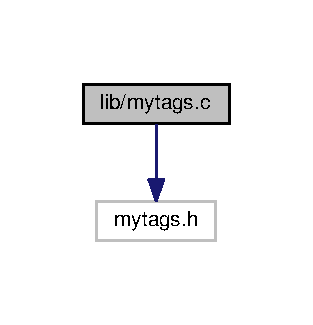
\includegraphics[width=150pt]{mytags_8c__incl}
\end{center}
\end{figure}
\subsection*{Classes}
\begin{DoxyCompactItemize}
\item 
struct \hyperlink{structtag}{tag}
\end{DoxyCompactItemize}
\subsection*{Functions}
\begin{DoxyCompactItemize}
\item 
Tag \hyperlink{mytags_8c_aaba7ed4551722063bfbc2e34b3f657ed}{init\+Tag} ()
\begin{DoxyCompactList}\small\item\em Inicializa uma Tag. \end{DoxyCompactList}\item 
Tag \hyperlink{mytags_8c_ac7296164bf5ca83d6f1a487fc55987e9}{create\+Tag} (long id, char $\ast$name)
\begin{DoxyCompactList}\small\item\em Cria uma Tag. \end{DoxyCompactList}\item 
long \hyperlink{mytags_8c_a3d33d8daebb69d85b40779c25dbbf378}{get\+Tag\+Id} (Tag t)
\begin{DoxyCompactList}\small\item\em Retorna o id de uma Tag. \end{DoxyCompactList}\item 
char $\ast$ \hyperlink{mytags_8c_ac5b9468b420ff068ca72dd4df27bf90f}{get\+Tag\+Name} (Tag t)
\begin{DoxyCompactList}\small\item\em Retorna a string com o nome da Tag. \end{DoxyCompactList}\item 
void \hyperlink{mytags_8c_a41c163d83371fa80c233c476f215668d}{free\+Tag} (void $\ast$t)
\begin{DoxyCompactList}\small\item\em Liberta a memória alocada por uma Tag. \end{DoxyCompactList}\end{DoxyCompactItemize}


\subsection{Detailed Description}
Ficheiro que contém a implementação das Tags. 



\subsection{Function Documentation}
\index{mytags.\+c@{mytags.\+c}!create\+Tag@{create\+Tag}}
\index{create\+Tag@{create\+Tag}!mytags.\+c@{mytags.\+c}}
\subsubsection[{\texorpdfstring{create\+Tag(long id, char $\ast$name)}{createTag(long id, char *name)}}]{\setlength{\rightskip}{0pt plus 5cm}Tag create\+Tag (
\begin{DoxyParamCaption}
\item[{long}]{id, }
\item[{char $\ast$}]{name}
\end{DoxyParamCaption}
)}\hypertarget{mytags_8c_ac7296164bf5ca83d6f1a487fc55987e9}{}\label{mytags_8c_ac7296164bf5ca83d6f1a487fc55987e9}


Cria uma Tag. 


\begin{DoxyParams}{Parameters}
{\em long} & id da Tag. \\
\hline
{\em char$\ast$} & string com o nome da Tag. \\
\hline
\end{DoxyParams}
\begin{DoxyReturn}{Returns}
Tag criada. 
\end{DoxyReturn}
\index{mytags.\+c@{mytags.\+c}!free\+Tag@{free\+Tag}}
\index{free\+Tag@{free\+Tag}!mytags.\+c@{mytags.\+c}}
\subsubsection[{\texorpdfstring{free\+Tag(void $\ast$t)}{freeTag(void *t)}}]{\setlength{\rightskip}{0pt plus 5cm}void free\+Tag (
\begin{DoxyParamCaption}
\item[{void $\ast$}]{t}
\end{DoxyParamCaption}
)}\hypertarget{mytags_8c_a41c163d83371fa80c233c476f215668d}{}\label{mytags_8c_a41c163d83371fa80c233c476f215668d}


Liberta a memória alocada por uma Tag. 


\begin{DoxyParams}{Parameters}
{\em void$\ast$} & apontador para a Tag a limpar da memória. \\
\hline
\end{DoxyParams}
\index{mytags.\+c@{mytags.\+c}!get\+Tag\+Id@{get\+Tag\+Id}}
\index{get\+Tag\+Id@{get\+Tag\+Id}!mytags.\+c@{mytags.\+c}}
\subsubsection[{\texorpdfstring{get\+Tag\+Id(\+Tag t)}{getTagId(Tag t)}}]{\setlength{\rightskip}{0pt plus 5cm}long get\+Tag\+Id (
\begin{DoxyParamCaption}
\item[{Tag}]{t}
\end{DoxyParamCaption}
)}\hypertarget{mytags_8c_a3d33d8daebb69d85b40779c25dbbf378}{}\label{mytags_8c_a3d33d8daebb69d85b40779c25dbbf378}


Retorna o id de uma Tag. 


\begin{DoxyParams}{Parameters}
{\em Tag} & tag. \\
\hline
\end{DoxyParams}
\begin{DoxyReturn}{Returns}
long id da Tag. 
\end{DoxyReturn}
\index{mytags.\+c@{mytags.\+c}!get\+Tag\+Name@{get\+Tag\+Name}}
\index{get\+Tag\+Name@{get\+Tag\+Name}!mytags.\+c@{mytags.\+c}}
\subsubsection[{\texorpdfstring{get\+Tag\+Name(\+Tag t)}{getTagName(Tag t)}}]{\setlength{\rightskip}{0pt plus 5cm}char$\ast$ get\+Tag\+Name (
\begin{DoxyParamCaption}
\item[{Tag}]{t}
\end{DoxyParamCaption}
)}\hypertarget{mytags_8c_ac5b9468b420ff068ca72dd4df27bf90f}{}\label{mytags_8c_ac5b9468b420ff068ca72dd4df27bf90f}


Retorna a string com o nome da Tag. 


\begin{DoxyParams}{Parameters}
{\em Tag} & tag. \\
\hline
\end{DoxyParams}
\begin{DoxyReturn}{Returns}
char$\ast$ string com o nome da Tag. 
\end{DoxyReturn}
\index{mytags.\+c@{mytags.\+c}!init\+Tag@{init\+Tag}}
\index{init\+Tag@{init\+Tag}!mytags.\+c@{mytags.\+c}}
\subsubsection[{\texorpdfstring{init\+Tag()}{initTag()}}]{\setlength{\rightskip}{0pt plus 5cm}Tag init\+Tag (
\begin{DoxyParamCaption}
{}
\end{DoxyParamCaption}
)}\hypertarget{mytags_8c_aaba7ed4551722063bfbc2e34b3f657ed}{}\label{mytags_8c_aaba7ed4551722063bfbc2e34b3f657ed}


Inicializa uma Tag. 

\begin{DoxyReturn}{Returns}
Tag inicializada. 
\end{DoxyReturn}

\hypertarget{util_8c}{}\section{lib/util.c File Reference}
\label{util_8c}\index{lib/util.\+c@{lib/util.\+c}}


Ficheiro que contém a implementação de estruturas e funções úteis para resolução de querys.  


{\ttfamily \#include \char`\"{}util.\+h\char`\"{}}\\*
Include dependency graph for util.\+c\+:
\nopagebreak
\begin{figure}[H]
\begin{center}
\leavevmode
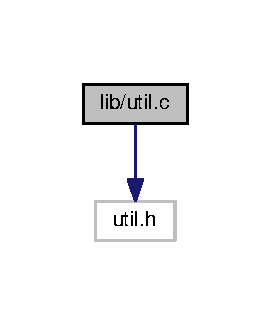
\includegraphics[width=130pt]{util_8c__incl}
\end{center}
\end{figure}
\subsection*{Classes}
\begin{DoxyCompactItemize}
\item 
struct \hyperlink{structrespostas}{respostas}
\item 
struct \hyperlink{structduplo}{duplo}
\end{DoxyCompactItemize}
\subsection*{Functions}
\begin{DoxyCompactItemize}
\item 
Res\+Post \hyperlink{util_8c_ae6f056f8633ec031784e23932c508d25}{init\+Res\+Post} (long pid)
\begin{DoxyCompactList}\small\item\em Retorna uma estrutura Res\+Post inicializada. \end{DoxyCompactList}\item 
Key \hyperlink{util_8c_a60434069ee0240fea86b5738cf6d7d21}{get\+Res\+Post\+Parent} (Res\+Post r)
\begin{DoxyCompactList}\small\item\em Retorna o ID guardado na estrutura. \end{DoxyCompactList}\item 
Heap \hyperlink{util_8c_a20739fe1a3e9cbdf9dd679c4c18854b3}{get\+Res\+Post\+Heap} (Res\+Post r)
\begin{DoxyCompactList}\small\item\em Retorna a heap guardada na estrutura. \end{DoxyCompactList}\item 
void {\bfseries free\+Res\+Post} (Res\+Post r)\hypertarget{util_8c_a448f9cc7803754e9ab585dbb1366bfa3}{}\label{util_8c_a448f9cc7803754e9ab585dbb1366bfa3}

\item 
L\+O\+N\+G\+\_\+list \hyperlink{util_8c_ab4474badc0ede23e8a7b095cca56ac3e}{init\+\_\+ll} (int N)
\begin{DoxyCompactList}\small\item\em Função que inicializa uma L\+O\+N\+G\+\_\+list. \end{DoxyCompactList}\item 
Duplos \hyperlink{util_8c_a4c5c29e5f165c0df9df3fda08b3e7d34}{init\+Duplos} (int N)
\begin{DoxyCompactList}\small\item\em Função que inicializa a estrutura Duplos. \end{DoxyCompactList}\item 
void \hyperlink{util_8c_a796d89b27b73c711760d6e40a330c868}{set\+\_\+duplos\+\_\+pos} (Duplos dup, int i)
\begin{DoxyCompactList}\small\item\em Função que altera o campo \char`\"{}pos\char`\"{} de um Duplos. \end{DoxyCompactList}\item 
Duplos \hyperlink{util_8c_a6ad5de0a44d77ff16ddec8257d141753}{set\+\_\+duplos\+\_\+tnum} (Duplos dup, T\+Num tn)
\begin{DoxyCompactList}\small\item\em Função que introduz um par Tag-\/\+Num em um Duplos. \end{DoxyCompactList}\item 
Duplos \hyperlink{util_8c_a85d927844a42e39f9ddc341fd1db7042}{insere\+\_\+\+Duplos} (L\+O\+N\+G\+\_\+list ll, T\+Num tn, int N, int i)
\begin{DoxyCompactList}\small\item\em Função cria e preenche os parâmetros de um Duplos. \end{DoxyCompactList}\item 
L\+O\+N\+G\+\_\+list \hyperlink{util_8c_aafa3001f0aac7709715f4059551f87a0}{get\+\_\+duplos\+\_\+ll} (Duplos dup)
\begin{DoxyCompactList}\small\item\em Função que retorna a L\+O\+N\+G\+\_\+list de um Duplos. \end{DoxyCompactList}\item 
T\+Num \hyperlink{util_8c_a625c56a7565e05e3bcffdd63134166a7}{get\+\_\+duplos\+\_\+tnum} (Duplos dup)
\begin{DoxyCompactList}\small\item\em Função que retorna um par Tag-\/\+Num de um Duplos. \end{DoxyCompactList}\item 
int \hyperlink{util_8c_a5a151853e521b4e046c678ea71abee7c}{get\+\_\+duplos\+\_\+pos} (Duplos dup)
\begin{DoxyCompactList}\small\item\em Função que retorna o parâmetro \textquotesingle{}pos\textquotesingle{} de um Duplos. \end{DoxyCompactList}\item 
char $\ast$$\ast$ \hyperlink{util_8c_a6a52cab09d93c8d5574a1380ab0891f7}{mystrdups} (char $\ast$$\ast$s)
\begin{DoxyCompactList}\small\item\em Função que copia um array de strings. \end{DoxyCompactList}\end{DoxyCompactItemize}


\subsection{Detailed Description}
Ficheiro que contém a implementação de estruturas e funções úteis para resolução de querys. 



\subsection{Function Documentation}
\index{util.\+c@{util.\+c}!get\+\_\+duplos\+\_\+ll@{get\+\_\+duplos\+\_\+ll}}
\index{get\+\_\+duplos\+\_\+ll@{get\+\_\+duplos\+\_\+ll}!util.\+c@{util.\+c}}
\subsubsection[{\texorpdfstring{get\+\_\+duplos\+\_\+ll(\+Duplos dup)}{get_duplos_ll(Duplos dup)}}]{\setlength{\rightskip}{0pt plus 5cm}L\+O\+N\+G\+\_\+list get\+\_\+duplos\+\_\+ll (
\begin{DoxyParamCaption}
\item[{Duplos}]{dup}
\end{DoxyParamCaption}
)}\hypertarget{util_8c_aafa3001f0aac7709715f4059551f87a0}{}\label{util_8c_aafa3001f0aac7709715f4059551f87a0}


Função que retorna a L\+O\+N\+G\+\_\+list de um Duplos. 


\begin{DoxyParams}{Parameters}
{\em Duplos} & duplo. return L\+O\+N\+G\+\_\+list do Duplos. \\
\hline
\end{DoxyParams}
\index{util.\+c@{util.\+c}!get\+\_\+duplos\+\_\+pos@{get\+\_\+duplos\+\_\+pos}}
\index{get\+\_\+duplos\+\_\+pos@{get\+\_\+duplos\+\_\+pos}!util.\+c@{util.\+c}}
\subsubsection[{\texorpdfstring{get\+\_\+duplos\+\_\+pos(\+Duplos dup)}{get_duplos_pos(Duplos dup)}}]{\setlength{\rightskip}{0pt plus 5cm}int get\+\_\+duplos\+\_\+pos (
\begin{DoxyParamCaption}
\item[{Duplos}]{dup}
\end{DoxyParamCaption}
)}\hypertarget{util_8c_a5a151853e521b4e046c678ea71abee7c}{}\label{util_8c_a5a151853e521b4e046c678ea71abee7c}


Função que retorna o parâmetro \textquotesingle{}pos\textquotesingle{} de um Duplos. 


\begin{DoxyParams}{Parameters}
{\em Duplos} & duplo. return int inteiro do parâmetro \textquotesingle{}pos\textquotesingle{} de um Duplos. \\
\hline
\end{DoxyParams}
\index{util.\+c@{util.\+c}!get\+\_\+duplos\+\_\+tnum@{get\+\_\+duplos\+\_\+tnum}}
\index{get\+\_\+duplos\+\_\+tnum@{get\+\_\+duplos\+\_\+tnum}!util.\+c@{util.\+c}}
\subsubsection[{\texorpdfstring{get\+\_\+duplos\+\_\+tnum(\+Duplos dup)}{get_duplos_tnum(Duplos dup)}}]{\setlength{\rightskip}{0pt plus 5cm}T\+Num get\+\_\+duplos\+\_\+tnum (
\begin{DoxyParamCaption}
\item[{Duplos}]{dup}
\end{DoxyParamCaption}
)}\hypertarget{util_8c_a625c56a7565e05e3bcffdd63134166a7}{}\label{util_8c_a625c56a7565e05e3bcffdd63134166a7}


Função que retorna um par Tag-\/\+Num de um Duplos. 


\begin{DoxyParams}{Parameters}
{\em Duplos} & duplo. return T\+Num par Tag-\/\+Num. \\
\hline
\end{DoxyParams}
\index{util.\+c@{util.\+c}!get\+Res\+Post\+Heap@{get\+Res\+Post\+Heap}}
\index{get\+Res\+Post\+Heap@{get\+Res\+Post\+Heap}!util.\+c@{util.\+c}}
\subsubsection[{\texorpdfstring{get\+Res\+Post\+Heap(\+Res\+Post r)}{getResPostHeap(ResPost r)}}]{\setlength{\rightskip}{0pt plus 5cm}Heap get\+Res\+Post\+Heap (
\begin{DoxyParamCaption}
\item[{Res\+Post}]{r}
\end{DoxyParamCaption}
)}\hypertarget{util_8c_a20739fe1a3e9cbdf9dd679c4c18854b3}{}\label{util_8c_a20739fe1a3e9cbdf9dd679c4c18854b3}


Retorna a heap guardada na estrutura. 


\begin{DoxyParams}{Parameters}
{\em Res\+Post.} & return Heap. \\
\hline
\end{DoxyParams}
\index{util.\+c@{util.\+c}!get\+Res\+Post\+Parent@{get\+Res\+Post\+Parent}}
\index{get\+Res\+Post\+Parent@{get\+Res\+Post\+Parent}!util.\+c@{util.\+c}}
\subsubsection[{\texorpdfstring{get\+Res\+Post\+Parent(\+Res\+Post r)}{getResPostParent(ResPost r)}}]{\setlength{\rightskip}{0pt plus 5cm}Key get\+Res\+Post\+Parent (
\begin{DoxyParamCaption}
\item[{Res\+Post}]{r}
\end{DoxyParamCaption}
)}\hypertarget{util_8c_a60434069ee0240fea86b5738cf6d7d21}{}\label{util_8c_a60434069ee0240fea86b5738cf6d7d21}


Retorna o ID guardado na estrutura. 


\begin{DoxyParams}{Parameters}
{\em Res\+Post.} & return Key ID. \\
\hline
\end{DoxyParams}
\index{util.\+c@{util.\+c}!init\+\_\+ll@{init\+\_\+ll}}
\index{init\+\_\+ll@{init\+\_\+ll}!util.\+c@{util.\+c}}
\subsubsection[{\texorpdfstring{init\+\_\+ll(int N)}{init_ll(int N)}}]{\setlength{\rightskip}{0pt plus 5cm}L\+O\+N\+G\+\_\+list init\+\_\+ll (
\begin{DoxyParamCaption}
\item[{int}]{N}
\end{DoxyParamCaption}
)}\hypertarget{util_8c_ab4474badc0ede23e8a7b095cca56ac3e}{}\label{util_8c_ab4474badc0ede23e8a7b095cca56ac3e}


Função que inicializa uma L\+O\+N\+G\+\_\+list. 


\begin{DoxyParams}{Parameters}
{\em int} & tamanho da L\+O\+N\+G\+\_\+list. return L\+O\+N\+G\+\_\+list criada e inicializada. \\
\hline
\end{DoxyParams}
\index{util.\+c@{util.\+c}!init\+Duplos@{init\+Duplos}}
\index{init\+Duplos@{init\+Duplos}!util.\+c@{util.\+c}}
\subsubsection[{\texorpdfstring{init\+Duplos(int N)}{initDuplos(int N)}}]{\setlength{\rightskip}{0pt plus 5cm}Duplos init\+Duplos (
\begin{DoxyParamCaption}
\item[{int}]{N}
\end{DoxyParamCaption}
)}\hypertarget{util_8c_a4c5c29e5f165c0df9df3fda08b3e7d34}{}\label{util_8c_a4c5c29e5f165c0df9df3fda08b3e7d34}


Função que inicializa a estrutura Duplos. 


\begin{DoxyParams}{Parameters}
{\em int} & tamanho da L\+O\+N\+G\+\_\+list do duplos. return Duplos inicializado \\
\hline
\end{DoxyParams}
\index{util.\+c@{util.\+c}!init\+Res\+Post@{init\+Res\+Post}}
\index{init\+Res\+Post@{init\+Res\+Post}!util.\+c@{util.\+c}}
\subsubsection[{\texorpdfstring{init\+Res\+Post(long pid)}{initResPost(long pid)}}]{\setlength{\rightskip}{0pt plus 5cm}Res\+Post init\+Res\+Post (
\begin{DoxyParamCaption}
\item[{long}]{pid}
\end{DoxyParamCaption}
)}\hypertarget{util_8c_ae6f056f8633ec031784e23932c508d25}{}\label{util_8c_ae6f056f8633ec031784e23932c508d25}


Retorna uma estrutura Res\+Post inicializada. 


\begin{DoxyParams}{Parameters}
{\em long} & id de uma pergunta. return Res\+Post estrutura inicializada. \\
\hline
\end{DoxyParams}
\index{util.\+c@{util.\+c}!insere\+\_\+\+Duplos@{insere\+\_\+\+Duplos}}
\index{insere\+\_\+\+Duplos@{insere\+\_\+\+Duplos}!util.\+c@{util.\+c}}
\subsubsection[{\texorpdfstring{insere\+\_\+\+Duplos(\+L\+O\+N\+G\+\_\+list ll, T\+Num tn, int N, int i)}{insere_Duplos(LONG_list ll, TNum tn, int N, int i)}}]{\setlength{\rightskip}{0pt plus 5cm}Duplos insere\+\_\+\+Duplos (
\begin{DoxyParamCaption}
\item[{L\+O\+N\+G\+\_\+list}]{ll, }
\item[{T\+Num}]{tn, }
\item[{int}]{N, }
\item[{int}]{i}
\end{DoxyParamCaption}
)}\hypertarget{util_8c_a85d927844a42e39f9ddc341fd1db7042}{}\label{util_8c_a85d927844a42e39f9ddc341fd1db7042}


Função cria e preenche os parâmetros de um Duplos. 


\begin{DoxyParams}{Parameters}
{\em L\+O\+N\+G\+\_\+list} & lista a ser introduzida. \\
\hline
{\em T\+Num} & par Tag-\/\+Num a ser introduzido. \\
\hline
{\em int} & tamanho da L\+O\+N\+G\+\_\+list. \\
\hline
{\em int} & índice a ser introduzido. return Duplos criado. \\
\hline
\end{DoxyParams}
\index{util.\+c@{util.\+c}!mystrdups@{mystrdups}}
\index{mystrdups@{mystrdups}!util.\+c@{util.\+c}}
\subsubsection[{\texorpdfstring{mystrdups(char $\ast$$\ast$s)}{mystrdups(char **s)}}]{\setlength{\rightskip}{0pt plus 5cm}char$\ast$$\ast$ mystrdups (
\begin{DoxyParamCaption}
\item[{char $\ast$$\ast$}]{s}
\end{DoxyParamCaption}
)}\hypertarget{util_8c_a6a52cab09d93c8d5574a1380ab0891f7}{}\label{util_8c_a6a52cab09d93c8d5574a1380ab0891f7}


Função que copia um array de strings. 


\begin{DoxyParams}{Parameters}
{\em char$\ast$$\ast$} & Array de strings. return char$\ast$$\ast$ Array de strings copiado. \\
\hline
\end{DoxyParams}
\index{util.\+c@{util.\+c}!set\+\_\+duplos\+\_\+pos@{set\+\_\+duplos\+\_\+pos}}
\index{set\+\_\+duplos\+\_\+pos@{set\+\_\+duplos\+\_\+pos}!util.\+c@{util.\+c}}
\subsubsection[{\texorpdfstring{set\+\_\+duplos\+\_\+pos(\+Duplos dup, int i)}{set_duplos_pos(Duplos dup, int i)}}]{\setlength{\rightskip}{0pt plus 5cm}void set\+\_\+duplos\+\_\+pos (
\begin{DoxyParamCaption}
\item[{Duplos}]{dup, }
\item[{int}]{i}
\end{DoxyParamCaption}
)}\hypertarget{util_8c_a796d89b27b73c711760d6e40a330c868}{}\label{util_8c_a796d89b27b73c711760d6e40a330c868}


Função que altera o campo \char`\"{}pos\char`\"{} de um Duplos. 


\begin{DoxyParams}{Parameters}
{\em int} & número a ser introduzido no campo \char`\"{}pos\char`\"{} do Duplos. \\
\hline
\end{DoxyParams}
\index{util.\+c@{util.\+c}!set\+\_\+duplos\+\_\+tnum@{set\+\_\+duplos\+\_\+tnum}}
\index{set\+\_\+duplos\+\_\+tnum@{set\+\_\+duplos\+\_\+tnum}!util.\+c@{util.\+c}}
\subsubsection[{\texorpdfstring{set\+\_\+duplos\+\_\+tnum(\+Duplos dup, T\+Num tn)}{set_duplos_tnum(Duplos dup, TNum tn)}}]{\setlength{\rightskip}{0pt plus 5cm}Duplos set\+\_\+duplos\+\_\+tnum (
\begin{DoxyParamCaption}
\item[{Duplos}]{dup, }
\item[{T\+Num}]{tn}
\end{DoxyParamCaption}
)}\hypertarget{util_8c_a6ad5de0a44d77ff16ddec8257d141753}{}\label{util_8c_a6ad5de0a44d77ff16ddec8257d141753}


Função que introduz um par Tag-\/\+Num em um Duplos. 


\begin{DoxyParams}{Parameters}
{\em Duplos} & duplo de L\+O\+N\+G\+\_\+list e T\+Num. return Duplos inicializado \\
\hline
\end{DoxyParams}

%--- End generated contents ---

% Index
\backmatter
\newpage
\phantomsection
\clearemptydoublepage
\addcontentsline{toc}{chapter}{Index}
\printindex

\end{document}
